 % This is samplepaper.tex, a sample chapter demonstrating the
% LLNCS macro package for Springer Computer Science proceedings;
% Version 2.20 of 2017/10/04
%
\documentclass[runningheads]{llncs}
%
% Used for displaying a sample figure. If possible, figure files should
% be included in EPS format.
% For language-specific hyphenations etc.
\usepackage[english]{babel}
% For subfigures
\usepackage{subcaption}
\usepackage{xcolor}
% For nice links
\usepackage{url}
% For playing with colors in tabular environments
\usepackage{colortbl}
% For math symbols, such as \nexists
\usepackage{amssymb}
% For more math symbols, such as \mapsfrom
\usepackage{stmaryrd}
% For advanced graphics
% For equations, arrays of equations, defining operator names, etc.
\usepackage{amsmath}
% For cursive math
\usepackage{mathrsfs}
% For math symbols, such as \nexists
\usepackage{amssymb}
%% For math environments, such as "definition"
%\usepackage{amsthm}
%\theoremstyle{definition}
%\newdefinition{definition}{Definition}[section]
%\newtheorem{theorem}{Theorem}[section]
% For enumerating the line numbers
\usepackage[left]{lineno}
% For diagonally-split fractions (\sfrac)
\usepackage{xfrac}
% For nice (diagonal) fractions
\usepackage{nicefrac}
% For side notes, missing figures and inline to-do's
\usepackage[textsize=scriptsize,backgroundcolor=yellow!40]{todonotes}
% Resize the width of todo-notes on the margins
%\setlength{\marginparwidth}{1.25cm}
% For specifying kewords and acronyms
\usepackage[nonumberlist,acronym,sanitize=none]{glossaries}
\glsdisablehyper
% For commenting out some parts of the text
\usepackage{comment}
% For hyperlinks
\usepackage[pdftex, colorlinks=true, hyperfootnotes=true, hyperindex=true,
            plainpages=false, pagebackref=false, pdfpagelabels=true, pdfstartview=FitH,
            linkcolor=blue, citecolor=blue, urlcolor=blue,
            bookmarks, bookmarksopen, bookmarksdepth=3]{hyperref}
% For smart references
\usepackage[capitalise,nameinlink]{cleveref}
% To have "Figure 3(a)" in place of "Figure 3a" and  "Table 3(a)" in place of "Table 3a"
\captionsetup[subfigure]{subrefformat=simple,labelformat=simple}
    \renewcommand\thesubfigure{(\alph{subfigure})}
\captionsetup[subtable]{subrefformat=simple,labelformat=simple}
    \renewcommand\thesubtable{(\alph{subtable})}
\crefname{algocf}{alg.}{algs.}
\Crefname{algocf}{Algorithm}{Algorithms}
\crefname{section}{Sect.}{Sects.} % Era un poco prolisso
% TikZ/Pgf advanced graphics
\usepackage{tkz-base}
\usetikzlibrary{decorations.pathmorphing,trees,snakes,arrows,shapes,automata,petri}
% To use inline and other fancy list-like environments (e.g., inparaenum)
\usepackage{paralist}
% To divide a text line into multiple columns
\usepackage{multicol}
% To create good-looking book-style tables
\usepackage{booktabs}
% To play around with list environments
\usepackage{enumitem}
% To create multirow cells in tables
\usepackage{multirow}
% To create rotated cells in tables
\usepackage{rotating}
% To create enumerated lists, whose numbering is reversed
\usepackage{etaremune}
%% To make algorithmic nice-looking pseudocode
% \usepackage[ruled,linesnumbered,algo2e]{algorithm2e}
%% For creating side-notes
\usepackage{marginnote}
% For superimposing symbols over one another within math env.
\usepackage{mathtools}
% For strange math symbols like \Dashv
\usepackage{mathabx}
% For adjusting the size of tables to the text width, if necessary: \begin{adjustbox}{max width=\textwidth}
\usepackage{adjustbox}
% For LaTeX if/then statements
\usepackage{ifthen}
% For strike-through cancellations
\usepackage[normalem]{ulem}
%% The lineno packages adds line numbers. Start line numbering with
%% \begin{linenumbers}, end it with \end{linenumbers}. Or switch it on
%% for the whole article with \linenumbers.
\usepackage{lineno}
% For highlighted text
\usepackage{soul}
% To put table environments and co. side by side
\usepackage{floatrow}
\floatsetup[table]{style=plaintop}
\usepackage{listings}
\begin{comment}
	contenuto...
\lstset{ %
%	backgroundcolor=\color{white},   % choose the background color; you must add \usepackage{color} or \usepackage{xcolor}; should come as last argument
	basicstyle=\tiny\ttfamily,       % the size of the fonts that are used for the code
	breakatwhitespace=true,          % sets if automatic breaks should only happen at whitespace
	breaklines=true,                 % sets automatic line breaking
	captionpos=b,                    % sets the caption-position to bottom
	commentstyle=\color{gray},       % comment style
%	escapeinside={\%*}{*)},          % if you want to add LaTeX within your code
	extendedchars=true,              % lets you use non-ASCII characters; for 8-bits encodings only, does not work with UTF-8
	frame=single,	                 % adds a frame around the code
	keepspaces=true,                 % keeps spaces in text, useful for keeping indentation of code (possibly needs columns=flexible)
%	keywordstyle=\color{blue},       % keyword style
%	language=SQL,                    % the language of the code
%	deletekeywords={Time},      % if you want to delete keywords from the given language
%	morekeywords={*,...},            % if you want to add more keywords to the set
	numbers=left,                    % where to put the line-numbers; possible values are (none, left, right)
	numbersep=5pt,                   % how far the line-numbers are from the code
	numberstyle=\tiny\color{gray}, % the style that is used for the line-numbers
%	rulecolor=\color{black},         % if not set, the frame-color may be changed on line-breaks within not-black text (e.g. comments (green here))
	showspaces=false,                % show spaces everywhere adding particular underscores; it overrides 'showstringspaces'
	showstringspaces=false,          % underline spaces within strings only
	showtabs=false,                  % show tabs within strings adding particular underscores
	stepnumber=1,                    % the step between two line-numbers. If it's 1, each line will be numbered
%	stringstyle=\color{mymauve},     % string literal style
	tabsize=2,	                   % sets default tabsize to 2 spaces
%	title=\lstname                   % show the filename of files included with \lstinputlisting; also try caption instead of title
	morecomment=[l]\%
}


\end{comment}

\lstset{
	backgroundcolor=\color{scriptcolor},
	extendedchars=true,
	basicstyle=\fontsize{8pt}{8pt}\selectfont\ttfamily,
	showstringspaces=false,
	showspaces=false,
%	linewidth=19em,
	numbers=left,
	numberstyle=\footnotesize,
	numbersep=5pt,
	tabsize=2,
	breaklines=true,
	showtabs=false,
	captionpos=b,
	belowskip=-0.2em,
	lineskip = 0.1em
}
\crefname{lstlisting}{Listing}{Listings}
% To add dummy text
\usepackage{lipsum}
% To have newlines in cells, with commands such as \makecell or \thead
\usepackage{makecell}
% For diagonal lines in tables
\usepackage{diagbox}
% For a decent formatting of numbers (and a wonderful system for numeric columns in tables, ``S'')
\usepackage[scientific-notation=false,group-separator={,}]{siunitx}
% To enable text protrusion
\usepackage{microtype}
% For footnote-references: \footref
\usepackage{footmisc}
% For side figures
\usepackage{wrapfig}
%
%\usepackage{xcolor}

\usepackage{listings}

\usepackage[T1]{fontenc}
\usepackage{lmodern}
% If you use the hyperref package, please uncomment the following line
% to display URLs in blue roman font according to Springer's eBook style:
\renewcommand\UrlFont{\color{blue}\rmfamily}
%
\definecolor{specializedcliniccolor}{RGB}{0, 153, 0}
\definecolor{pharmacolor}{RGB}{0, 110, 175}% Define a custom color (in this case, red)
\newcommand{\Actor}[1]{\textsf{#1}}
\newcommand{\Compo}[1]{\texttt{#1}}
\newcommand{\Activ}[1]{\textrm{#1}}
%
\usepackage{orcidlink}
%% Saving trees -- put this in the preamble
\usepackage{newtxtext}
%% Do not let the Times package affect the monospaced font (Courier is utterly ugly)
\renewcommand{\ttdefault}{cmtt}
%% Shrinking white space here and there…
\usepackage[subtle]{savetrees}
%\addtolength{\topmargin}{-1\baselineskip} % Careful!
%\addtolength{\textheight}{2\baselineskip} % Careful!
%% save space around floats (tables, algo's, fig's):
\setlength{\textfloatsep}{15pt}% Reduce \textfloatsep
%% save more space by suppressing vertical space between paragraphs
%\parskip1pt
%% To remove the starting indentation in footnotes.
% \deffootnote{0.5em}{0em}{\textsuperscript{\thefootnotemark}\,}
% Customize cleveref format for enumerate items
\crefformat{enumi}{#2\textup{#1}#3}



\newenvironment{leftbox}[1]
 {\itemize[
    nosep,
    leftmargin=0pt,
    rightmargin=\dimexpr\textwidth-#1\relax,
    itemindent=\parindent,
    listparindent=\parindent,
  ]\item[]\relax}
 {\enditemize}

\newenvironment{rightbox}[1]
 {\itemize[
    nosep,
    leftmargin=\dimexpr\textwidth-#1\relax,
    rightmargin=0pt,
    itemindent=\parindent,
    listparindent=\parindent,
  ]\item[]\relax}
 {\enditemize}
\begin{document}
%
\title{Preserving Data Secrecy in Decentralized \\ Inter-organizational Process Mining}
%
\titlerunning{Data Secrecy in Decentralized Inter-organizational Process Mining}
% If the paper title is too long for the running head, you can set
% an abbreviated paper title here
%
\author{%
Valerio~Goretti\inst{1}\orcidlink{0000-0001-9714-4278} \and %\inst{1}\orcidID{0000-0001-9714-4278} \and 
Davide~Basile\inst{1}\orcidlink{0000-1111-2222-3333} \and %\inst{1}\orcidID{0000-1111-2222-3333} \and
Luca~Barbaro\inst{1}\orcidlink{0000-0002-2975-5330} \and %\inst{1}\orcidID{0000-0002-2975-5330} \and
Claudio~Di~Ciccio\inst{1,2}\orcidlink{0000-0001-5570-0475}%\inst{1}\orcidID{0000-0001-5570-0475}}
}
%
\authorrunning{V.\ Goretti, D.\ Basile, L.\ Barbaro, C.\ Di Ciccio}
% First names are abbreviated in the running head.
% If there are more than two authors, 'et al.' is used.
%
\institute{Sapienza University of Rome, Italy, \email{\href{mailto:davide.basile@uniroma1.it;luca.barbaro@uniroma1.it;valerio.goretti@uniroma1.it;claudio.diciccio@uniroma1.it}{name.surname@uniroma1.it}}
\and
Utrecht University, Netherlands}%, \email{\href{mailto:c.diciccio@uu.nl}{c.diciccio@uu.nl}}}
%
\maketitle

\begin{abstract}
 Inter-organizational business processes involve multiple independent organizations collaborating to achieve mutual interests. 
Process mining techniques have the potential to allow these organizations to enhance operational efficiency, improve performance, and deepen the understanding of their business based on the recorded process event data. 
However, inter-organizational process mining faces substantial challenges, including topical secrecy concerns: The involved organizations may not be willing to expose their own data to run mining algorithms jointly with their counterparts or third parties. 
In this paper, we introduce a novel approach that unlocks process mining on multiple actors' process event data while safeguarding the secrecy and integrity of the original records in an inter-organizational business setting.
To ensure that the data acquisition, merging and elaboration phases are secure and that the processed information is hidden from involved and external actors alike, our approach resorts to decentralized trusted applications running in Trusted Execution Environments (TEEs).
We show the feasibility of our solution by showcasing its application to a healthcare scenario.
%
\begin{comment}% Original abstract
 Through process mining tecniques, organizations enhances their operational efficiency, improve performances, and deepen the understanding of their business processes. While most process mining research focuses on intra-organizational settings, the emerging importance of inter-organizational collaborations for operational excellence cannot be ignored. Inter-organizational business processes involve multiple independent organizations collaborating to achieve mutual interests. However, inter-organizational process mining faces substantial challenges, primarily centered on confidentiality concerns. In this paper, we introduce a novel approach based on the adoption of trusted applications running in Trusted Execution Environments (TEEs). Our research work aims at ensuring privacy preservation and safeguarding the integrity of sensitive information during process mining procedures in inter-organizational contexts. Therefore, we introduce a TEE-based infrastructure supporting the execution of trusted applications through which partner organizations securely share operational information and apply process mining techniques. We show the feasibility of our solution by exposing an healthcare scenario that serve as running example. Our contribution includes a discussion of the proposed research work that addresses strengths and areas for improvement.
\end{comment}

 \keywords{%
 	Collaborative information systems architectures
 	\and
 	Trusted execution environments
 	\and
 	Confidential computing%
 }
\end{abstract}

\linenumbers

\section{Introduction}
\label{sec:introduction}
\begin{comment}
\todo[inline]{%
	´CDC: Status corrente secondo me. Abbiamo\ldots
	Un'intro affabile ma che dobbiamo ricalibrare per toglierla dal pantano della TEE e puntare dritto al nostro obiettivo dichiarato e mantenuto, con vista sul potenziale inespresso.\\
	Un motivating scenario che però resta staccato dal resto.\\
	Un related work che però dovrebbe spostarsi sul far capire cosa facciamo di più e di diverso, o di simile ma rivisto.\\
	Una overview eccellente dell'architettura che però non è connessa con l'esempio.\\
	Una overview accurata delle interazioni dei moduli (e quando lo spazio è poco è il caso di fare il merge tra le due cose per risparmiare spazio, come ci dicemmo) -- anche qui senza esempio, dunque capire cosa si fa dove è arduo. Non per me o per te, ma perché conosciamo il lavoro. Chi non lo conosce, non ha assolutamente idea di cosa voglia dire fare il merge degli eventi da tracce provienienti da actor diversi rimettendoli in ordine così da preservare integrità temporale, per esempio.\\
	Una discussion/evaluation ben congegnata in cui però manca la parte quantitativa e la qualitativa è ancora da dettagliare.\\
	Una conclusione.%
}
\end{comment}
In today's business landscape, organizations constantly seek ways to enhance operational efficiency, increase performance, and gain valuable insights to improve their processes. Process mining offers techniques to discover, monitor, and improve business processes by extracting knowledge from chronological records known as \textit{event logs} \cite{van2012process}. Organizations record in these ledgers events referring to activities and interactions occurring within a business process. The vast majority of process mining contributions consider \textit{intra-organizational} settings, in which business processes are executed inside individual organizations. However, organizations increasingly recognize the value of collaboration and synergy in achieving operational excellence. \textit{Inter-organizational} business processes involve several independent organizations cooperating to achieve a shared objective \cite{van2011intra}. Despite the advantages of transparency, performance optimization, and benchmarking that companies can gain from such practices, inter-organizational process mining raises challenges that make it still hardly applicable. The major issue concerns confidentiality. Companies are reluctant to outsource to their partners inside information that is required to execute process mining algorithms. Indeed, the sharing of sensitive operational data across organizational boundaries introduces concerns about data privacy, security, and compliance with regulations. \textit{Trusted Execution Environments} (TEEs) can serve as fundamental enablers to balance the need for insights with the imperative to protect sensitive information in inter-organizational settings. TEEs offer secure contexts that guarantee code integrity and data confidentiality in external devices. \textit{Trusted applications} are tamper-proof software objects running in these environments. 

In this paper, we propose the CONFINE framework for inter-organizational process mining. It resorts to trusted applications to preserve the secrecy and integrity of shared data. To pursue this aim, we design a decentralized software architecture for a four-staged protocol: (i) The initial exchange of preliminary metadata, (ii) The attestation of the miner entity, (iii) the secure transmission of encrypted data amid multiple parties, (iiii) The privacy-preserving merge of the shared information segments followed by the isolated and verifiable computation of process discovery algorithms on joined data.
We evaluate our proof-of-concept implementation against synthetic and real-world-based data with a convergence test and memory effectiveness assessment.

The remainder of the paper is structured as follows: \cref{sec:background} provides an overview of related work inherent to the theme of inter-organizational process mining. In \cref{sec:motivating}, we introduce a use case example that considers a healthcare scenario. The CONFINE architecture is presented in \cref{sec:design}. Following on from this, we instantiate the addressed design principles in \cref{sec:realization}, focusing on the employed technologies, communication protocol, and implementation. In \cref{sec:evaluation}, we discuss our solution. Finally, we conclude and present directions for future work in \cref{sec:conclusion}.

\section{Related Work}
\todo[inline]{It can be reduced. EDIT: Already reduced. MISSING: what do we do similarly to and what do we do differently from / improve on the cited papers? A comparison is offered only with the work of M{\"u}ller et al.}
\label{sec:background}
%First inspiration work
% Inter-organizational and process mining
\begin{comment}
The work of M{\"u}ller et al.~\cite{muller2021process} is the first contribution that considers TEEs in combination with blockchain technologies for process mining purposes. This research proposes a conceptual architecture in which process mining algorithms are executed inside centralized third-party services. Inspired by this preliminary contribution, we design a decentralized approach context where each organization can run process mining algorithms without involving external stakeholders.
The literature proposes several studies that consider process mining techniques in inter-organizational environments. Van Der Aalst~\cite{van2011intra} shows that inter-organizational processes can be divided according to different dimensions making identifiable challenges of inter-organizational process extractions. Elkoumy et al.~\cite{elkoumy2020shareprom} propose a tool that allows independent parts of an organization to perform process mining operations by revealing only the result. This tool is called Shareprom and exploits the features of secure multi-party computation (MPC). Engel et al.~\cite{engel2016analyzing} present EDImine Framework, which allows to apply process mining operations for inter-organizational processes supported by the EDI standard\footnote{https://edicomgroup.com/learning-center/edi/standards} and evaluate their performance using business information.
Elkoumy et al.~\cite{elkoumy2020secure} propose an MPC-based architecture that aims to perform process mining operations without sharing their data or trusting third parties.
% inter-organizational and merge log
Applying process mining techniques in intra-organizational contexts requires merging the event logs of the organizations participating in the process. The literature offers several studies in this area. For instance, Hernandez-Resendiz et al.~\cite{hernandez2021merging} present a methodology for merging logs at the trace and activity level using rules and methods to discover the process. Claes et al.~\cite{claes2014merging} provide techniques for performing merge operations in inter-organizational environments. This paper indicates rules for merging data in order to perform process mining algorithms.
%data exchange 
The state of the art provides some studies that investigate issues and possible solutions regarding data exchange, more specifically in an business collaboration context. EDI standards enable the communication of business documents. Among these standards, the notion of process is not explicitly specified. This inhibits organizations from applying Business Process Management (BPM) methods in business collaboration environments. Engel et al.\cite{engel2011process} extended process mining techniques by discovering interaction sequences between business partners based on EDI exchanged documents. Lo et al.\cite{lo2020flexible} have provided and developed a framework for data exchange designed even in intra-organizational situations. This framework is based on blockchain and decentralized public key infrastructure technologies, which ensure scalability, reliability, data security, and data privacy.
% Use of data from other organizations(or person) integrity ecc ecc (LOCAL)
Additionally, there are several papers that propose solutions for the correct sharing and use of data by third parties. Xie et al.\cite{XIE2023321} propose an architecture for the internet of things based on TEE and blockchain. The proposed architecture aims to solve data and identity security problems in the process of data sharing. Basile et al.~\cite{Basile_Blockchain_based_resource_governance_for_decentralized_web_environments} in their study created a framework called ReGov that allows the exchange of sensitive information in a decentralized web context, ensuring usage control-based data access and usage. In order to control the consumer's device ReGov uses TEE that allows storage and utilization management of retrieved resources. Hussain et al.\cite{hussain2021sharing} present a tool for privacy protection and data management among multiple collaborating companies. This tool allows data encryption to be configured according to the privacy obligations dictated by the context of a system's use. 

\end{comment}

\todo[inline]{Our work revolves around the following areas: 1, 2 and 3. Next, we position our contribution against the existing body of literature.}

The work of M{\"u}ller et al.~\cite{muller2021process} is the first contribution that considers TEEs in combination with %blockchain technologies for process mining purposes.
process mining techniques.
% \todo{When do we use blockchain in this paper? If we do not use it, then we should make clear why we do not. Isn't it also the first paper that uses TEE for process mining? If it is, then we omit this blockchain thing and take it back for future work perhaps or as an additional detail.}
This research proposes a conceptual architecture in which process mining algorithms are executed inside centralized third-party services. Inspired by this preliminary contribution, we design a decentralized approach context where each organization can run process mining algorithms without involving external stakeholders. The theme of inter-organizational process mining is discussed in the literature from different perspectives. Van der Aalst~\cite{van2011intra} highlights the challenges of inter-organizational process extraction through a categorization. Elkoumy et al.~\cite{elkoumy2020shareprom} introduce Shareprom, a secure tool for inter-organizational process mining based on secure multi-party computation (MPC). Engel et al.~\cite{engel2016analyzing} present the EDImine Framework, which applies process mining to inter-organizational processes using the EDI standard. In inter-organizational contexts, merging event logs from different organizations is essential. Hernandez-Resendiz et al.~\cite{hernandez2021merging} propose a methodology for log merging, while Claes et al.~\cite{claes2014merging} provide techniques for merging data to support process mining algorithms. Data exchange in business collaboration environments has already been explored in various works. Engel et al.~\cite{engel2011process} extend process mining by analyzing interaction sequences based on EDI documents. Lo et al.~\cite{lo2020flexible} present a blockchain-based framework for secure data exchange, even within inter-organizational scenarios. Lastly, there are solutions for secure data sharing with third parties. Xie et al.~\cite{XIE2023321} propose an IoT architecture using TEE and blockchain. Basile et al.~\cite{Basile_Blockchain_based_resource_governance_for_decentralized_web_environments} introduce ReGov for controlled data utilization in decentralized web contexts.% Hussain et al.~\cite{hussain2021sharing} offers a tool for privacy protection and data management in collaborative settings, allowing data encryption to align with privacy requirements.
In the fast-evolving landscape of healthcare, seamless collaboration between multiple organizations is essential to ensure the highest standard of patient care. We delve into the application of Trusted Execution Environment (TEE) to facilitate the secure exchange of event logs between three pivotal actors: an esteemed hospital, a specialized clinic, and a leading pharmaceutical company. This innovative approach fosters a robust and trustworthy ecosystem where sensitive patient data can be shared securely, promoting seamless collaboration for the betterment of patient outcomes.

\section{Design}\label{sec:design}

In this section, we present the high-level architecture of our CONFINE framework. We consider the main functionalities of each component, avoiding details on the employed technologies discussed in the next sections. After introducing the architecture, we focus on the \Compo{Secure Miner}, a core component of our contribution.

\subsection{CONFINE architecture at large}
Our architecture involves different organizational ecosystems characterized by one or more machines. An organization may take at least one of the following roles: 
\begin{inparadesc}
\item[provisioning] if it delivers local event logs to be collaboratively mined;
\item[mining] if it applies process mining algorithms using event logs retrieved from provisioners.
\end{inparadesc}
% Provisioners collaborate to achieve common objectives and compose inter-organizational business processes whose event logs are scattered across multiple places. 
% Provisioners produce event logs, recording the operations executed to complete their part in the inter-organizational business process.
In \cref{fig:architecture_diagram}, we propose the high-level schematization of our solution.
In our solution, every organization hosts one or more \Compo{Node}s. Depending on the played role, \Compo{Node}s come endowed with a \Compo{Provisioner} or a \Compo{Secure Miner} component, or both. The \Compo{Provisioner} component consists of the following two main sub-components. The \begin{inparadesc}
\item[\Compo{Log Recorder}] registers the events taking place in the organizations' systems. The
\item[\Compo{Log Provider}] delivers on-demand data to mining players.
\end{inparadesc}
The \Actor{Hospital} (as well the other parties in our running example) records Alice and Bob's traces using the \Compo{Log Recorder}. The \Compo{Log Recorder} is queried by the \Compo{Log Provider} for event logs to be made available for mining. The latter controls access to local event logs by authenticating data requests by miners and rejecting those that come from unauthorized parties.
In our motivating scenario, the \Actor{Specialized clinic}, \Actor{Pharmaceutical company}, and the \Actor{Hospital} leverage \Compo{Log Provider}s to authenticate the miner party before sending their logs.  The \Compo{Secure Miner} component
% \Compo{Log Provider}s reject demands from unauthorized parties and only permit \texttt{Secure Miners} to use the data. 
% The \Compo{Secure Miner} 
shelters external event logs inside a protected environment to preserve data confidentiality and integrity.
Notice that \Compo{Log Provider}s accept requests issued solely by \Compo{Secure Miner}s. 
Next, we provide an in-depth focus on the latter.
% We provide an in-depth focus on this key component in the following.
\begin{comment}
\begin{figure}[t]
	\centering
	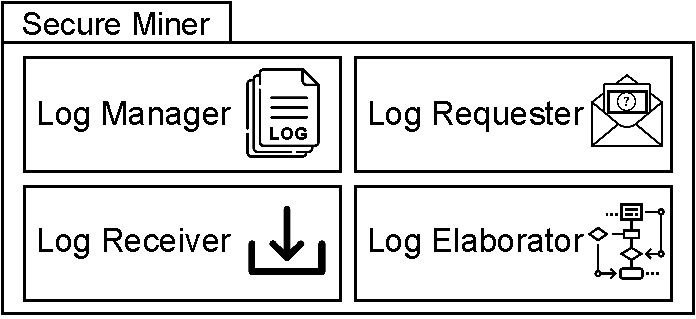
\includegraphics[width=0.5\linewidth]{content/figures/secureminersad.pdf}
	\caption{Subcomponents of the Secure Miner.}
	\label{fig:trusted_miner}
\end{figure}
\end{comment}

\begin{figure}[t]
	\centering
	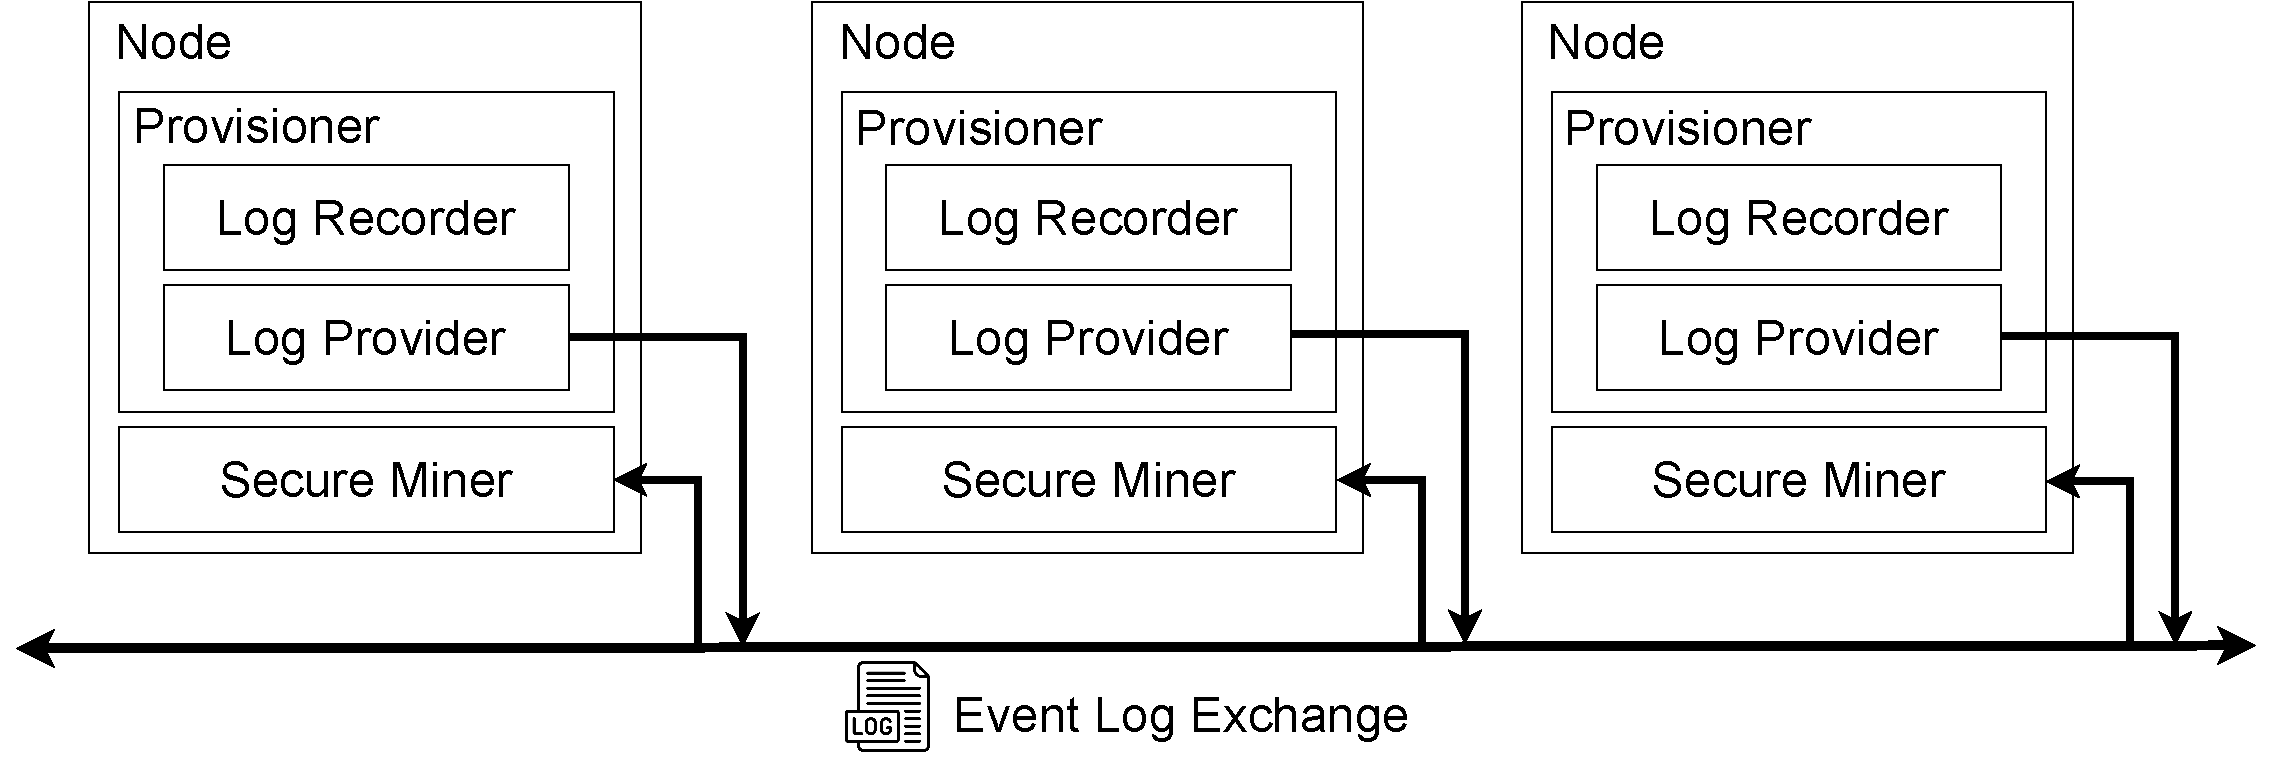
\includegraphics[width=0.79\linewidth]{content/figures/architecturediagram.pdf}
	\caption{High-level architectural overview.}
	\label{fig:architecture_diagram}
\end{figure}

\begin{wrapfigure}[9]{r}{0.4\textwidth}
	\vspace{-2em}
	\centering
	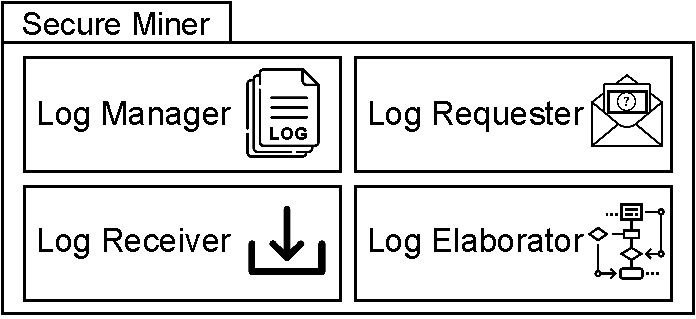
\includegraphics[width=1\textwidth]{content/figures/secureminersad.pdf}
	\caption[A gull]{Sub-components of the \\Secure Miner.}
	\label{fig:trusted_miner}
	\vspace{-6pt}
\end{wrapfigure} 
\subsection{Secure Miner}
The primary objective of the \Compo{Secure Miner} is to allow miners to securely execute process mining algorithms using event logs retrieved from provisioners such as the \Actor{Specialized clinic}, \Actor{Pharmaceutical company}, and the \Actor{Hospital} of our running example. \Compo{Secure Miner}s are isolated components that guarantee data inalterability and confidentiality. In \cref{fig:trusted_miner}, we show a schematization of the \Compo{Secure Miner}, which consists of four sub-components:
\begin{inparaenum}[\itshape(i)\upshape]
    \item The \Compo{Log Requester};
    \item The \Compo{Log Receiver};
    \item The \Compo{Log Manager}; 
    \item The \Compo{Log Elaborator}.
\end{inparaenum}
%Event logs belonging to provisioners are locked in the \Compo{Secure Miner}.
%We handle  data via the 
The \Compo{Log Requester} and the \Compo{Log Receiver} are the sub-components that we employ during the event log retrieval. \Compo{Log Requester}s send authenticable data requests to the \Compo{Log Provider} component of provisioners. The \Compo{Log Receiver} collects event logs sent by \texttt{Log Providers} and entrusts them to the \Compo{Log Manager}, securing them from accesses that are external to the \Compo{Secure Miner}.
Miners of our motivating scenario, such as the \Actor{University} and the \Actor{National Institute of Statistics}, employ these three components to retrieve and store Alice and Bob's data. The \Compo{Log Elaborator} merges the event data locked in the \Compo{Secure Miner} to have a global view of the inter-organizational process comprehensive of activities executed by each involved party. Thereupon, it executes process mining algorithms in a protected environment, inaccessible from the outside computation environment.
In our motivating scenario, the \Compo{Log Elaborator} combines the traces of Alice (i.e., $T^H_{312}$, $T^S_{312}$, and $T^C_{312}$) and Bob (i.e, $T^H_{711}$, $T^S_{711}$, and $T^C_{711}$), generates the chronologically sorted traces $T_{312}$ and $T_{711}$, and feeds them into the mining algorithms (see the bottom-right quadrant of \cref{tab:trace}).




\section{Realization}
\label{sec:realization}
%Focus generale sulle tecnologie utilizzate
In this section, we outline the technical aspects concerning the realization of our approach. Therefore we first present the enabler technologies through which we instantiate the design principles presented in \cref{sec:design}. After that, we discuss the interaction workflow between the instantiated technologies. Finally, we show the implementation details.

\subsection{Deployment}
As follows, we bridge the gap between high-level system architecture and its practical realization. \cref{fig:deployment_diagram} depicts a \textit{UML deployment diagram} \cite{koch2002expressive} that aims to help with understanding the instantiated infrastructure. 

%The \texttt{Organization Machine} represents the physical computation \textit{device} embracing the software and hardware entities of the company. The \texttt{Log Recorder}, the \texttt{Log Provider}, and \texttt{Secure Miner} are included in the \texttt{Organization Machine} as abstract \textit{components}. These logical elements incorporate the core functionalities already discussed in \cref{sec:design}. The \texttt{Organization Machine} is characterized by two \textit{execution environment}s, namely the \texttt{Operative System} and the \texttt{TEE}.
In our solution, we make a differentiation between the computational \textit{devices} designated for mining, denoted as \Compo{Miner Machine}s, and those specifically associated with provisioners, identified as \Compo{Provisioner Machine}s. To enhance clarity, we maintain the separation of these devices in the accompanying diagram. However, organizations have the flexibility to opt for integrated technologies that incorporate both mining and provisioning functionalities. %The \Compo{Miner Machine} encompasses the \Compo{Secure Miner} as an abstract component, incorporating its core functionalities, which we presented in detail in \cref{sec:design}. Similarly, the \Compo{Provisioner Machine} includes both the \Compo{Log Recorder} and the \Compo{Log Provider} as abstract components.
We included the \texttt{Log Recorder}, the \texttt{Log Provider}, and \texttt{Secure Miner} (already discussed in \cref{sec:design}) as abstract \textit{components} of the diagram, whose manifestation are described as follow. 

%\Compo{Provisioner Machine}s encompasses \Compo{Log Recorder}s and \Compo{Log Provider}s (already introduced in \cref{sec:design}) as abstract components, incorporating their core functionalities aimed at generating and transmitting event logs. We manifest the \texttt{Log Recorder} in the Process Aware Information System (\Compo{PAIS}) of the organization. These systems help users to handle business processes, including accounting and resource management \cite{Dumas.etal/2018:FundamentalsofBPM}. In our solution, the \texttt{PAIS} provides the \texttt{Log Server} access to event logs. \texttt{Log Servers} implements the functionalities of the \Compo{Log Provider} throigh web services that process remote data request and provides event log to miners. We build \Compo{Log Server}s upon existing web standards such as HTTP\footnote{\url{https://www.w3.org/Protocols/rfc2616/rfc2616.html}. Accessed: \today.}, FTP\footnote{\url{https://www.w3.org/Protocols/rfc959/}. Accessed: \today.}, and Goopher\footnote{\url{https://datatracker.ietf.org/doc/html/rfc1436}. Accessed: \today.}. \Compo{PAIS} and \Compo{Log Server} run on top of the \Compo{Operating System} of the \Compo{Provisioner Machine}.


\Compo{Provisioner Machine}s encompasses \Compo{Log Recorder}s and \Compo{Log Provider}s incorporating their core functionalities aimed at generating and transmitting event logs. Within the organizational context, we manifest the \Compo{Log Recorder} in the Process Aware Information System (\Compo{PAIS}), which plays a crucial role in managing various business processes, including accounting and resource management \cite{Dumas.etal/2018:FundamentalsofBPM}. 
\begin{figure}[t]
	\centering
	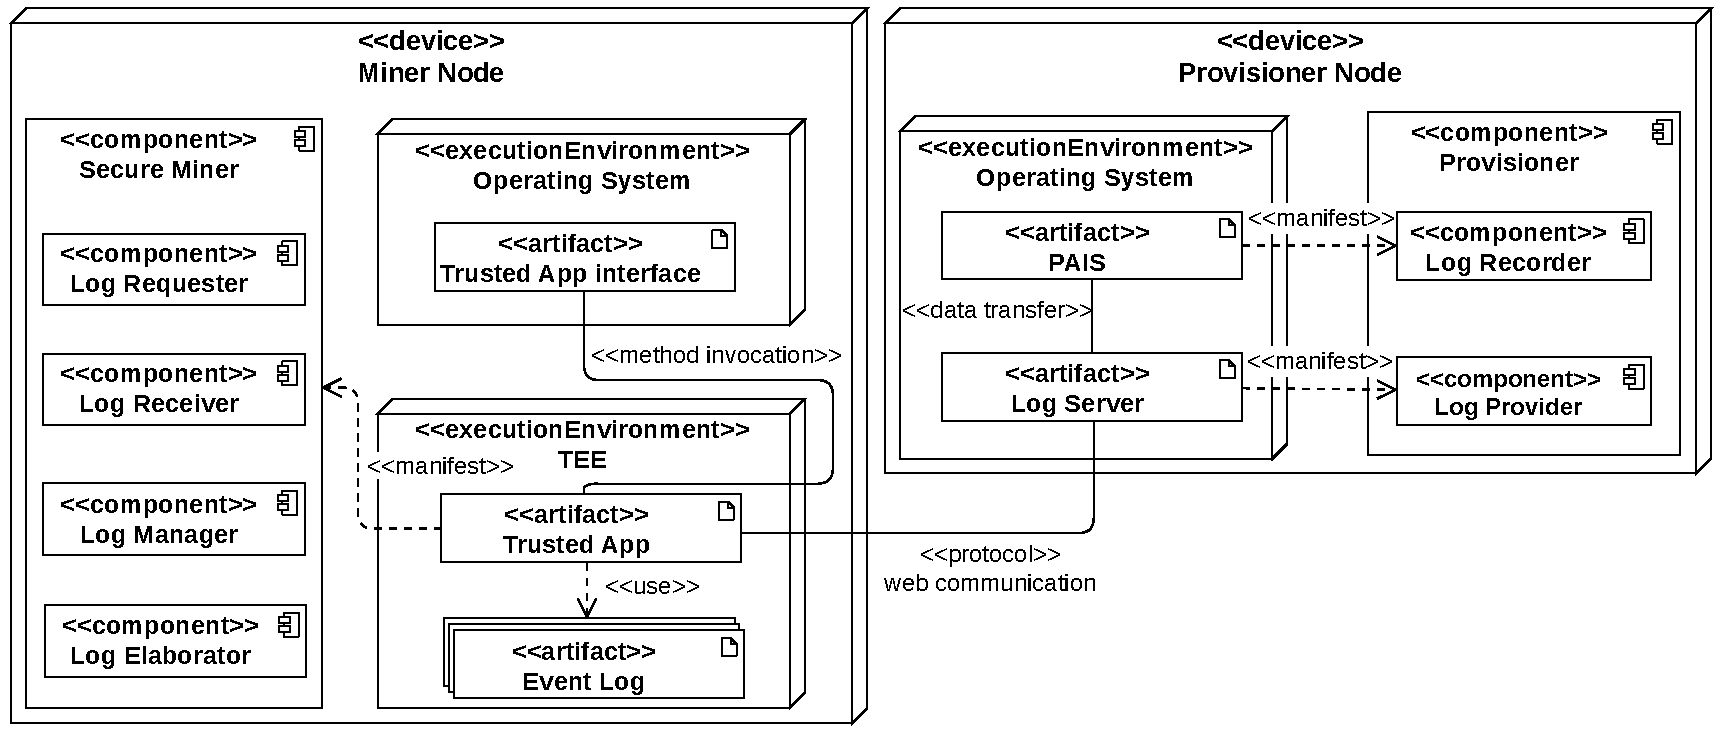
\includegraphics[width=1\linewidth]{content/figures/deploymentdiagram3.pdf}
	\caption{UML deployment diagram.}
	\label{fig:deployment_diagram}
\end{figure}
In our solution, the \Compo{PAIS} grants access to the \Compo{Log Server}, enabling it to retrieve event logs. The \Compo{Log Server}, on the other hand, embody the functionalities of the \Compo{Log Provider}, implementing web services amied at handling remote data requests and providing event logs to miners. \Compo{Log Servers} adheres to established web standards such as HTTP\footnote{\url{https://www.w3.org/Protocols/rfc2616/rfc2616.html}}, FTP\footnote{\url{https://www.w3.org/Protocols/rfc959/}}, and Goopher\footnote{\url{https://datatracker.ietf.org/doc/html/rfc1436}}. Both the \Compo{PAIS} and \Compo{Log Server} run on the top the \Compo{Operating System} of the \Compo{Provisioner Machine}.



%The \Compo{Miner Machine} is characterized by two \textit{execution environment}s, namely the \Compo{Operative System} and the \Compo{TEE}. \Compo{TEE}s create a separated context from the normal \Compo{Operating System} to protect code and data through an hardware-based encryption mechanism. \Compo{TEE}s relies on specific functionalities of the \Compo{Miner Machine}'s CPU that is capable of manage encrypted data in a reserved zone of the RAM\cite{citeTEEhere}. We leverage the security guarantees offered by these technologies to isolate a  \Compo{Trusted App} that fulfills the functionalities of the \Compo{Secure Miner} and its subcomponents. The \Compo{Trusted App} collects the logic to generate verifiable data requests, receive external event logs, store them in the \Compo{TEE}, and apply process mining algorithms. Procedures executed by the \Compo{Trusted App} are tamperproof. The \Compo{TEE} ensures that the code of the \Compo{Trusted App} executed within it is protected from malicious manipulations and unauthorized access from entities running inside the \Compo{Operating System}. Furthermore, we employ the isolated environment of \Compo{TEE} to store \Compo{Event Log}s of provisioner organizations inside the \Compo{Miner Machine}. The \texttt{TEE} provides a mechanism to protect this sensitive information without exposing it to the \Compo{Operative System}. The \Compo{Trusted App} is the only entity that can access the \Compo{Event Log}s, and feed them to process mining algorithms. Users can communicate with the \Compo{Trusted App} via the \Compo{Trusted App Interface}. The \Compo{Trusted Application} offers secure methods to safely receive information from the \Compo{Operative System} and outsource the outputs of the computation. These methods are invoked by the \Compo{Trusted App Interface} instantiating the only communication channel with the \texttt{Trusted App}.

The \Compo{Miner Machine} is characterized by two distinct \textit{execution environments}: the \Compo{Operating System} and the Trusted Execution Environment (\Compo{TEE}). \Compo{TEE}s establish an isolated context separate from the normal \Compo{Operating System}, safeguarding code and data through hardware-based encryption mechanisms. This technology relies on specialized components of the \Compo{Miner Machine}'s CPU capable of managing encrypted data within a reserved section of RAM \cite{TEEHERE}. We leverage the security guarantees provided by \Compo{TEE}s to isolate a \Compo{Trusted App} responsible for fulfilling the functions of the \Compo{ Secure Miner} and its associated subcomponents. The \Compo{Trusted App} consolidates the logic required for generating verifiable data requests, receiving external event logs, securely storing them within the \Compo{TEE}, and executing process mining algorithms. All procedures executed by the \Compo{Trusted App} are tamper-proof. The \Compo{TEE} ensures the integrity of the \Compo{Trusted App} code, protecting it against malicious manipulations and unauthorized access by entities operating within the \Compo{Operating System}. Additionally, we utilize the isolated environment of the \Compo{TEE} to securely store event logs from provisioner organizations within the \Compo{ Miner Machine}. The \Compo{TEE} safeguards this sensitive information alongside a unique asymetric key couple used for attestation purposes (i.e., public and private keys), preventing exposure to the \Compo{Operating System}. Access to data located in the \Compo{TEE} is restricted solely to the \Compo{Trusted App}. Users interact with the \Compo{Trusted App} through the \Compo{Trusted App Interface}, which serves as the exclusive communication channel. The \Compo{Trusted App} offers secure methods, invoked by the \Compo{Trusted App Interface}, for safely receiving information from the \Compo{Operating System} and outsourcing the results of computations, maintaining a high level of data security.

The interaction between the newly introduced technologies is elucidated as follows.
\begin{comment}
\begin{figure}[t]
\centering
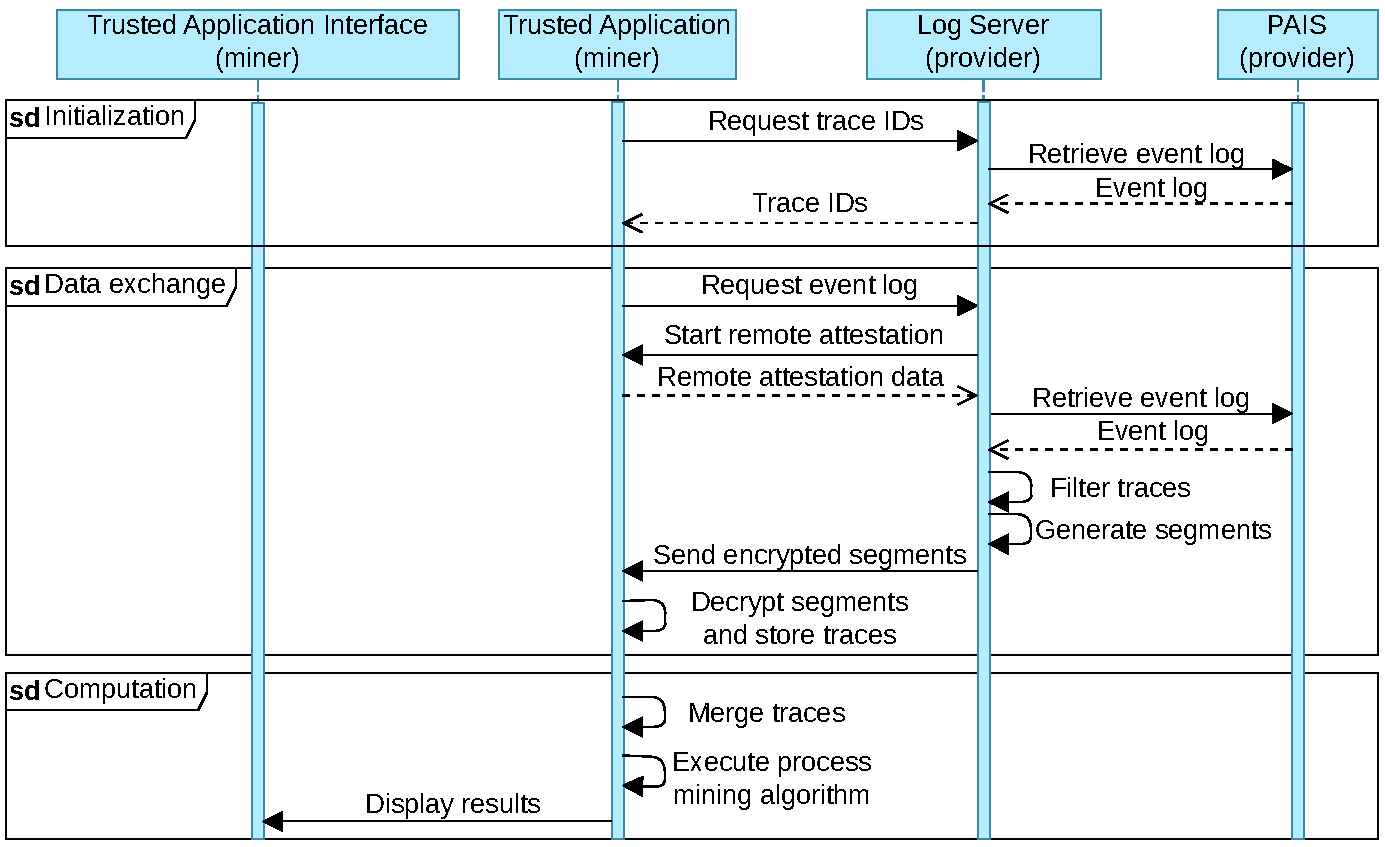
\includegraphics[width=0.9\linewidth]{content/figures/sequencediagram.pdf}
\caption{UML sequence diagram.}
\label{fig:sequence_diagram}
\end{figure}
\end{comment}
%orizontale

    \begin{figure}[t]
     \subfloat[][Initialization]{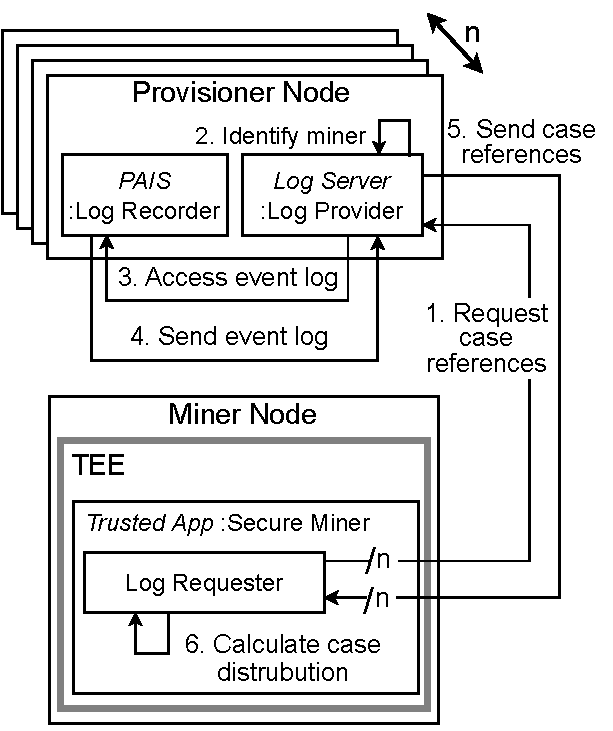
\includegraphics[width=0.29\linewidth]{content/figures/initializationworkflow.pdf}}\label{<figure1>}\hfill
     \subfloat[][Remote Attestation]{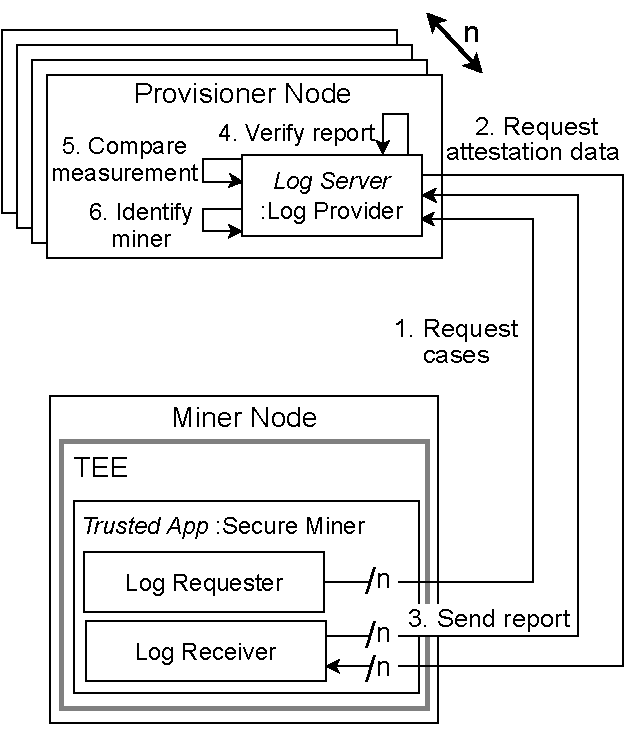
\includegraphics[width=0.32\linewidth]{content/figures/attestationworkflow.pdf}}\label{<figure1>}\hfill
     \subfloat[][Data Transmission]{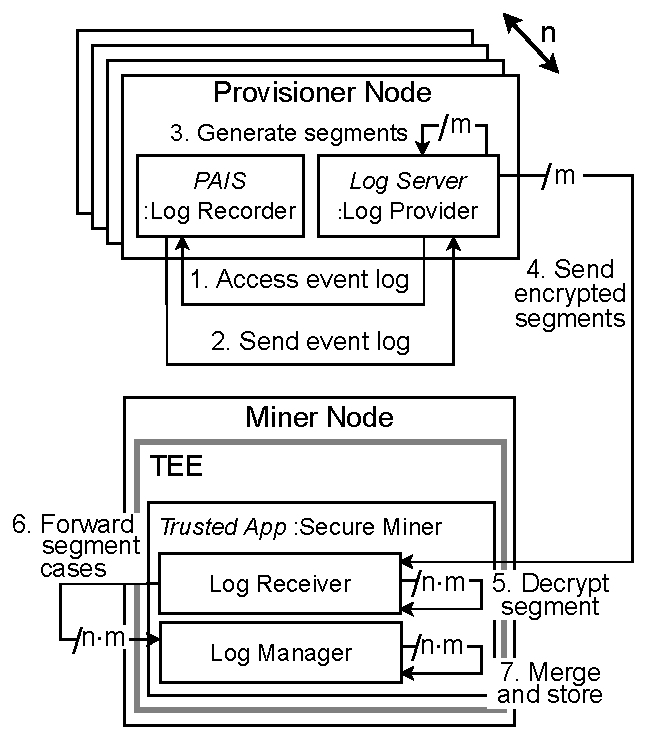
\includegraphics[width=0.33\linewidth]{content/figures/datatransmissionworkflow.pdf}}\label{<figure1>}\hfill
%     \subfloat[][Computation]{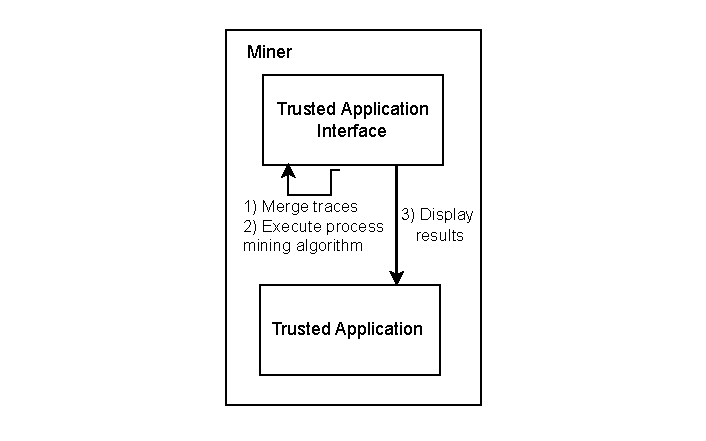
\includegraphics[width=0.32\linewidth]{content/figures/flow_computation.pdf}}\label{<figure1>}
     \caption{Schematization of the initialization, remote attestation and data transmission phase.}
     \label{flow}
    \end{figure}


\subsection{Workflow}
%

%
We separate the workflow into subsequent processes, namely \textit{initialization},\textit{remote attestation}, \textit{data transmission}, and \textit{computation}.
The parties involved in the workflow are a miner (i.e., an organization that executes process mining algorithms) and one or more providers (i.e., partner organizations that serve their event logs). %We distinguish three different phases of the process namely the \textit{initialization}, the \textit{data exchange}, and the \textit{computation}.
%\todo{CDC: We need an example. We must provide an example of (simplified) event log excerpt, with a few traces taken from the scenario, show which bits reside in the different machines, and show the final merged event log. Then, discuss it during the description of the workflow, showing how we get from the original pieces to the final one. This description takes time.}

\textbf{Initialization.} In the initialization, the miner's \texttt{Trusted Application} requests preliminary information from the providers' \texttt{Log Server} concerning the event logs of an inter-organizational business process. After authenticating the sender, the involved \texttt{Log Server}s retrieve the local event log from the \texttt{PAIS} and respond to the miner by providing the list of trace IDs in the event log. Hence, the \texttt{Trusted Application} collects the responses and stores them in the \texttt{TEE}.

\textbf{Remote Attestation.} \todo[inline]{Talk specifically of remote attestation}

\textbf{Data Transmission.} Once recorded the preliminary information, the miner starts the data exchange. Therefore, its \texttt{Trusted Application} sends data requests to the \texttt{Log Servers}. The requests include as parameters the list of trace ids and the segment size. Subsequently, the \texttt{Log Server}s starts the \textit{remote attestation} procedure, thanks to which they can verify that the sender of the log request: is a \texttt{Trusted Application} running inside a \texttt{TEE}; comes from a partner organization. This operation involves the exchange of additional messages between the \texttt{Log Server} and the \texttt{Trusted Application}. If the procedure is successful, the miner's identity is verified.
Subsequently, the \texttt{Log Servers} retrieve the local event log and filter its traces according to the trace IDs sent by the \texttt{Trusted Application}. Filtered event logs are split into several segments containing traces whose dimension does not exceed the segment size parameter. \texttt{Log Servers} encrypts the segments and send each of them to the \texttt{Trusted Application}. The \texttt{Trusted Application} decrypts the received segments, extracts the traces, and stores them in \texttt{Event Log}s inside the \texttt{TEE}.

\begin{wrapfigure}[9]{r}{0.33\textwidth}
   \vspace{-2em}
  \centering
  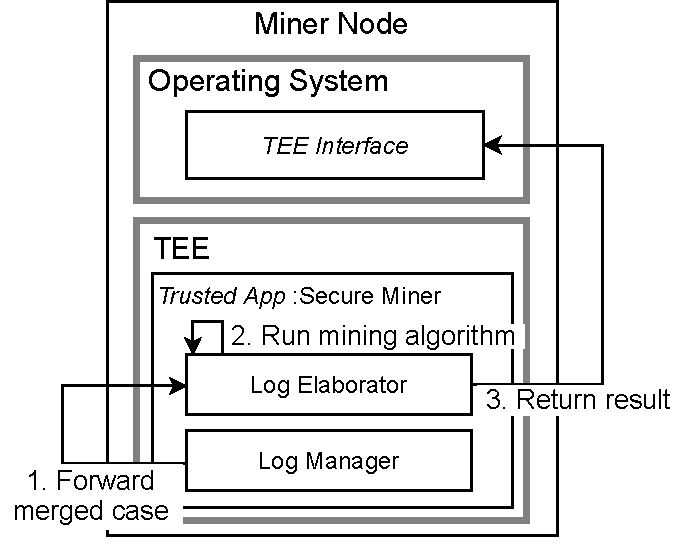
\includegraphics[width=1\textwidth]{content/figures/computationworkflow.pdf}
  \caption[A gull]{Schematization of the computation phase.}
  \vspace{-6pt}
\end{wrapfigure}
\textbf{Computation.} To start a computation routine, the \texttt{Trusted Application} needs all partner organizations to have delivered traces having the same ID. When this occurs, the \texttt{Trusted Application} merges external traces with the owned one. Assembled traces are used as parameters of process mining algorithms executed by the \texttt{Trusted Application} that presents the computation results to the users via the \texttt{Trusted Application Interface}.







\subsection{Implementation}
\label{sec:implementation:details}
In this section, we expound the implementation of our paper. The proposed implementation integrates a trusted application within a secure execution environment, complemented by the inclusion of event logs to address the issue outlined in the motivating scenario. The source code is accessible at the following URL: \url{https://github.com/dave0909/TEExProcessMining/}.


To realize the implementation of trusted applications, we employed EGo,\footnote{https://www.edgeless.systems/products/ego/} a framework designed for encoding trusted application in the Go\footnote{https://go.dev} programming language. Contained within the trusted application is the \Compo{Secure Miner} module, which facilitates the requisition, administration, and processing of logs from external organizations. To exemplify our approach's capability for conducting process analysis, we implemented a renowned process discovery algorithm within the \Compo{Secure Miner}. 










\begin{comment}
In this section, we describe the implementation of our paper. The implementation proposed integrates a trusted application running in a trusted execution environment and some event logs generated to address the solution proposed in the motivating scenario. The code is available at the following address: \url{https://github.com/dave0909/TEExProcessMining/}

We have encoded a well-known process discovery algorithm within the \texttt{Secure Miner} component to demonstrate the capability of conducting process analytics tasks with our approach.
To implement the trusted applications, we used the EGo,%
\footnote{https://www.edgeless.systems/products/ego/} 
a framework to encode programs for TEEs in %. EGo makes it possible to develop trusted applications programmed in 
GO.%
\footnote{https://go.dev}
% We developed the Trusted Application (TA) within the TEE with the same language. 
Within the TA there is the ``Secure Miner" module, which allows logs from other organizations to be requested, managed, and processed. Log processing is made possible by the implementation of the ``Heuristc Miner" process mining algorithm\ref{weijters2006process}, which takes the log traces as input and performs a discovery operation.
The output of the algorithm is a PNML\footnote{https://www.pnml.org}(Petri Net Markup Language) which allows the representation of Petri nets that graphically illustrate the model calculated by the algorithm. 
%The output of the algorithm is a file with the extension '.pnml'. PNML\footnote{https://www.pnml.org}(Petri Net Markup Language) is a markup language that allows the representation of Petri nets that graphically illustrate the model calculated by the algorithm. 
In order to generate the graphic image of the Petri net, we used the WoPed\footnote{https://woped.dhbw-karlsruhe.de} software, which takes as input a PNML file and provides the graphic representation of the Petri net. 

%Log provider language
Another fundamental module within the TA is the Log Provider. We wrote this part of TA in Go. The log provider is listening for log requests from other organizations on one of the ports set by the owning organization. When an organization decides to start the mining process, it requests the logs of the other organizations. The log providers accepts requests made by the organization that starting the mining operation and forwards its log.
\end{comment}

\label{sec:discussion:subsec:convergence}

\section{Discussion}
\label{sec:evaluation}

\begin{comment}
\todo[inline]{CDC: MISSING:
Nella evaluation, dobbiamo riportare l'uso di memoria qui conta perché è un parametro fondamentale.
\\
Dobbiamo informare il lettore sulle caratteristiche del log (numero eventi, numero tracce, dimensione totale in KB una volta salvato in formato XES), come lo abbiamo creato, perché il modello non è uguale a quello di Fig. 1.}
\end{comment}


In this section, we evaluate the proposed approach. The primary objective of the \cref{sec:discussion:subsec:convergence} is to delve into a convergence analysis by evaluating the efficacy of the collaborative data exchange process. We then took into assessment the memory usage by measuring the RAM usage in diverse parameter configurations in \cref{sec:discussion:subsec:memory}. In \cref{sec:discussion:subsec:validation}, we validate the addressed approach using real-world data to conclude the discussion. 

\subsection{Datasets}
\begin{comment}
\todo[inline]{the following text was in the implementation and was moved here }
In order to generate the logs for the execution of the trusted application, we produced a simulation model based on our running example (see~\cref{sec:motivating}).% was created based on BPMN notation\footnote{https://www.bpmn.org}. Subsequently, the model was imported fed as input into the BIMP tool.%
\footnote{https://bimp.cs.ut.ee}
% which made it possible to generate the synthetic event logs. 
The number of log traces generated through BIMP aligns with other works in the state of the art; the generation software was set to 1000 traces.
\todo{Mention Sepsis here}
Following the generation, the synthetic event log relating to the process model was filtered via ProM.%
\footnote{https://promtools.org}
We were able to filter the logs based on attribute values, which allowed us to filter the synthetic log according to the resource involved in the activities. Referring to the motivating scenario, the resources involved are the hospital, the specialized clinic, and the pharmaceutical company. In this way, we created three separate event logs from the initial event log, which were used to exchange data between the organizations.
\end{comment}
\begin{figure}[t]
	\subfloat[][Workflow net mined from the log of Pharmaceutical company.]{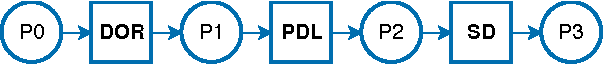
\includegraphics[width=0.37\linewidth]{content/figures/pharma_dep1.pdf}\label{fig:wfnet:a}}
	\hfill
	\subfloat[][Workflow net mined from the log of Specialized clinic.]{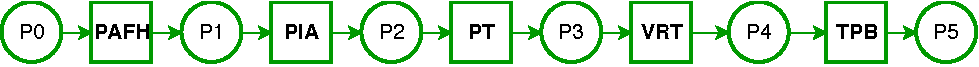
\includegraphics[width=0.57\linewidth]{content/figures/specialised_dep1.pdf}\label{fig:wfnet:b}}
	\hfill
	\vspace{1em}
	\subfloat[][Workflow net mined from the log of Hospital.]{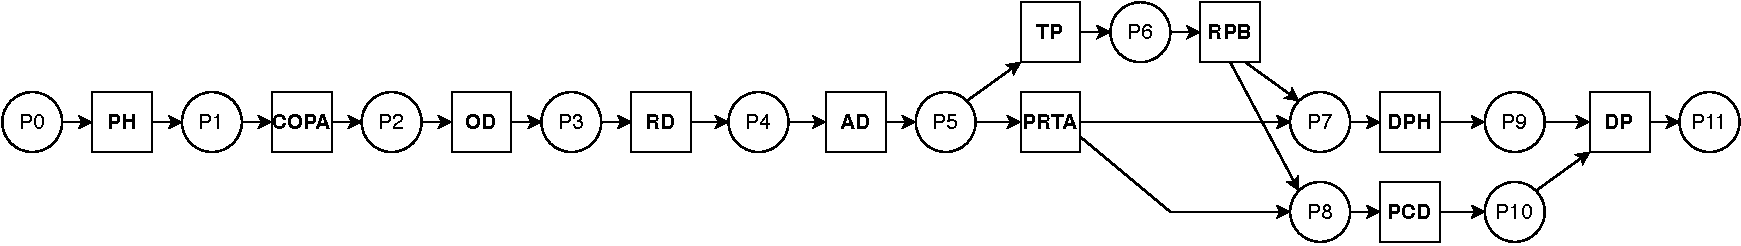
\includegraphics[width=1\linewidth]{content/figures/hospital_dep1.pdf}\label{fig:wfnet:c}}
	\hfill
	\vspace{1em}
	\subfloat[][Workflow net mined from the merged log in inter-organizational setting.]{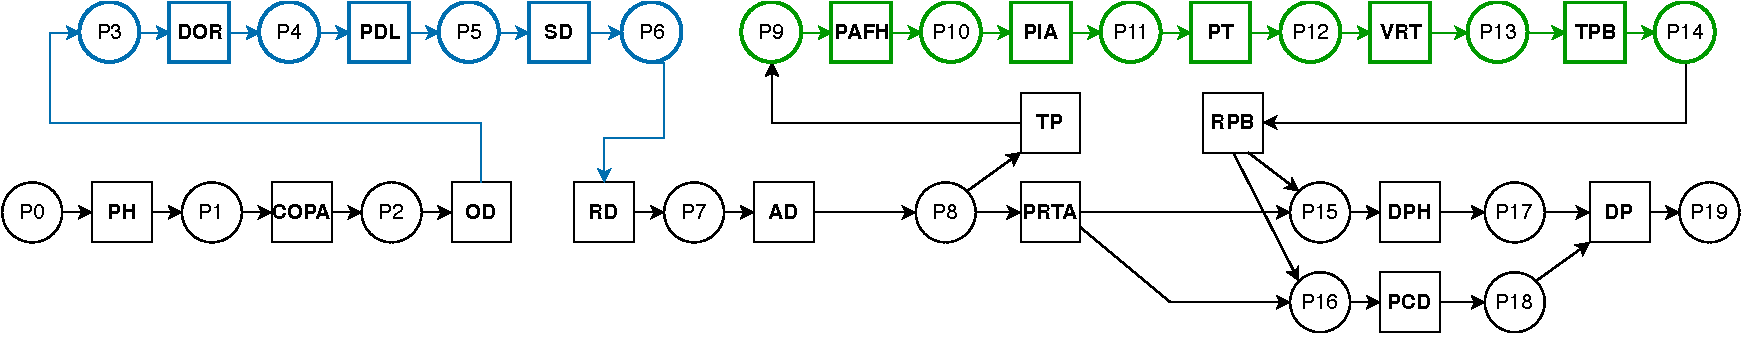
\includegraphics[width=1\linewidth]{content/figures/merged_dep1.pdf}\label{fig:wfnet:d}}
	\caption{Outputs used for the convergence test.}
	\label{fig:wfnet}
\end{figure}
\subsection{Convergence}
\label{sec:discussion:subsec:convergence}  
%\todo[inline]{Dobbiamo informare il lettore sulle caratteristiche del log (numero eventi, numero tracce, dimensione totale in KB una volta salvato in formato XES), come lo abbiamo creato, perché il modello non è uguale a quello di Fig. 1.}

We take into analysis the convergence of the process discovery outputs, as a way of validating the correct operation of the event log exchange mechanism, . Specifically, we generated the workflow nets computed in an intra-organizational setting, in which each organization directly mines its own event log. Subsequently, we employed our approach with a miner actor that computes the same discovery algorithm using an inter-organizational event log obtained as a result of the log exchange and the merging mechanisms. To run the test, we used the synthetic event logs devised from our motivating scenario whose BPMN is depicted in \cref{fig:BPMN_Healthcare}. The size of the \texttt{Hospital}, \texttt{Specialized clinic}, and \texttt{Pharmaceutical company} event logs are 4.8 MB, 1.1 MB, and 1.6 MB respectively.  Each log contains the standard value of 1000 traces, in accordance with the Sepsis Cases \cite{sepsis} event log. Upon visual examination of \cref{fig:wfnet}, we observe that the workflow net computed through our approach, displayed in \cref{fig:wfnet:d}, encapsulates the structure and behavior of the workflow nets derived from the intra-organizational discovery procedures depicted in \cref{fig:wfnet:a},\cref{fig:wfnet:b}, and \cref{fig:wfnet:c}. % Transitions and places within both workflow nets exhibit a clear congruence, indicative of a shared underlying process model. 
In detail, \cref{fig:wfnet:a}, colored in blue, depicts the process of the \texttt{pharmaceutical company} from the moment the drug order is received to its fulfillment. \Cref{fig:wfnet:b}, colored in green, depicts the process of the \texttt{Specialized clinic} from the moment the patient arrives from the \texttt{Hospital} to his transfer.
%This congruence further extends to the temporal sequencing of events and the causal relationships among process steps. This substantial resemblance between the two Workflow Nets serves as a testament to the seamless convergence of disparate event logs, achieved through the secure exchange mechanism. The fact that the collaborative process model, represented by the Workflow Net generated from the merged event log, aligns closely with the independent models of individual organizations underscores the fidelity and accuracy of the data exchange process.
% We point out that there are some minor changes between the process model behind the logs used for the tests and the BPMN in \cref{fig:BPMN_Healthcare}. To generate a log that allows us to simulate an inter-organizational scenario, it is necessary to make some simplifications to the presented BPMN syntax. Hence, we explain the slight inconsistencies between the process depicted in the motivating scenario and the process drawn by the workflow net of the test.



\subsection{Memory Usage}
\begin{comment}
\todo[inline]{grafici memory usage: segment size, }
\label{sec:discussion:subsec:memory}

\begin{figure}[t]
\centering
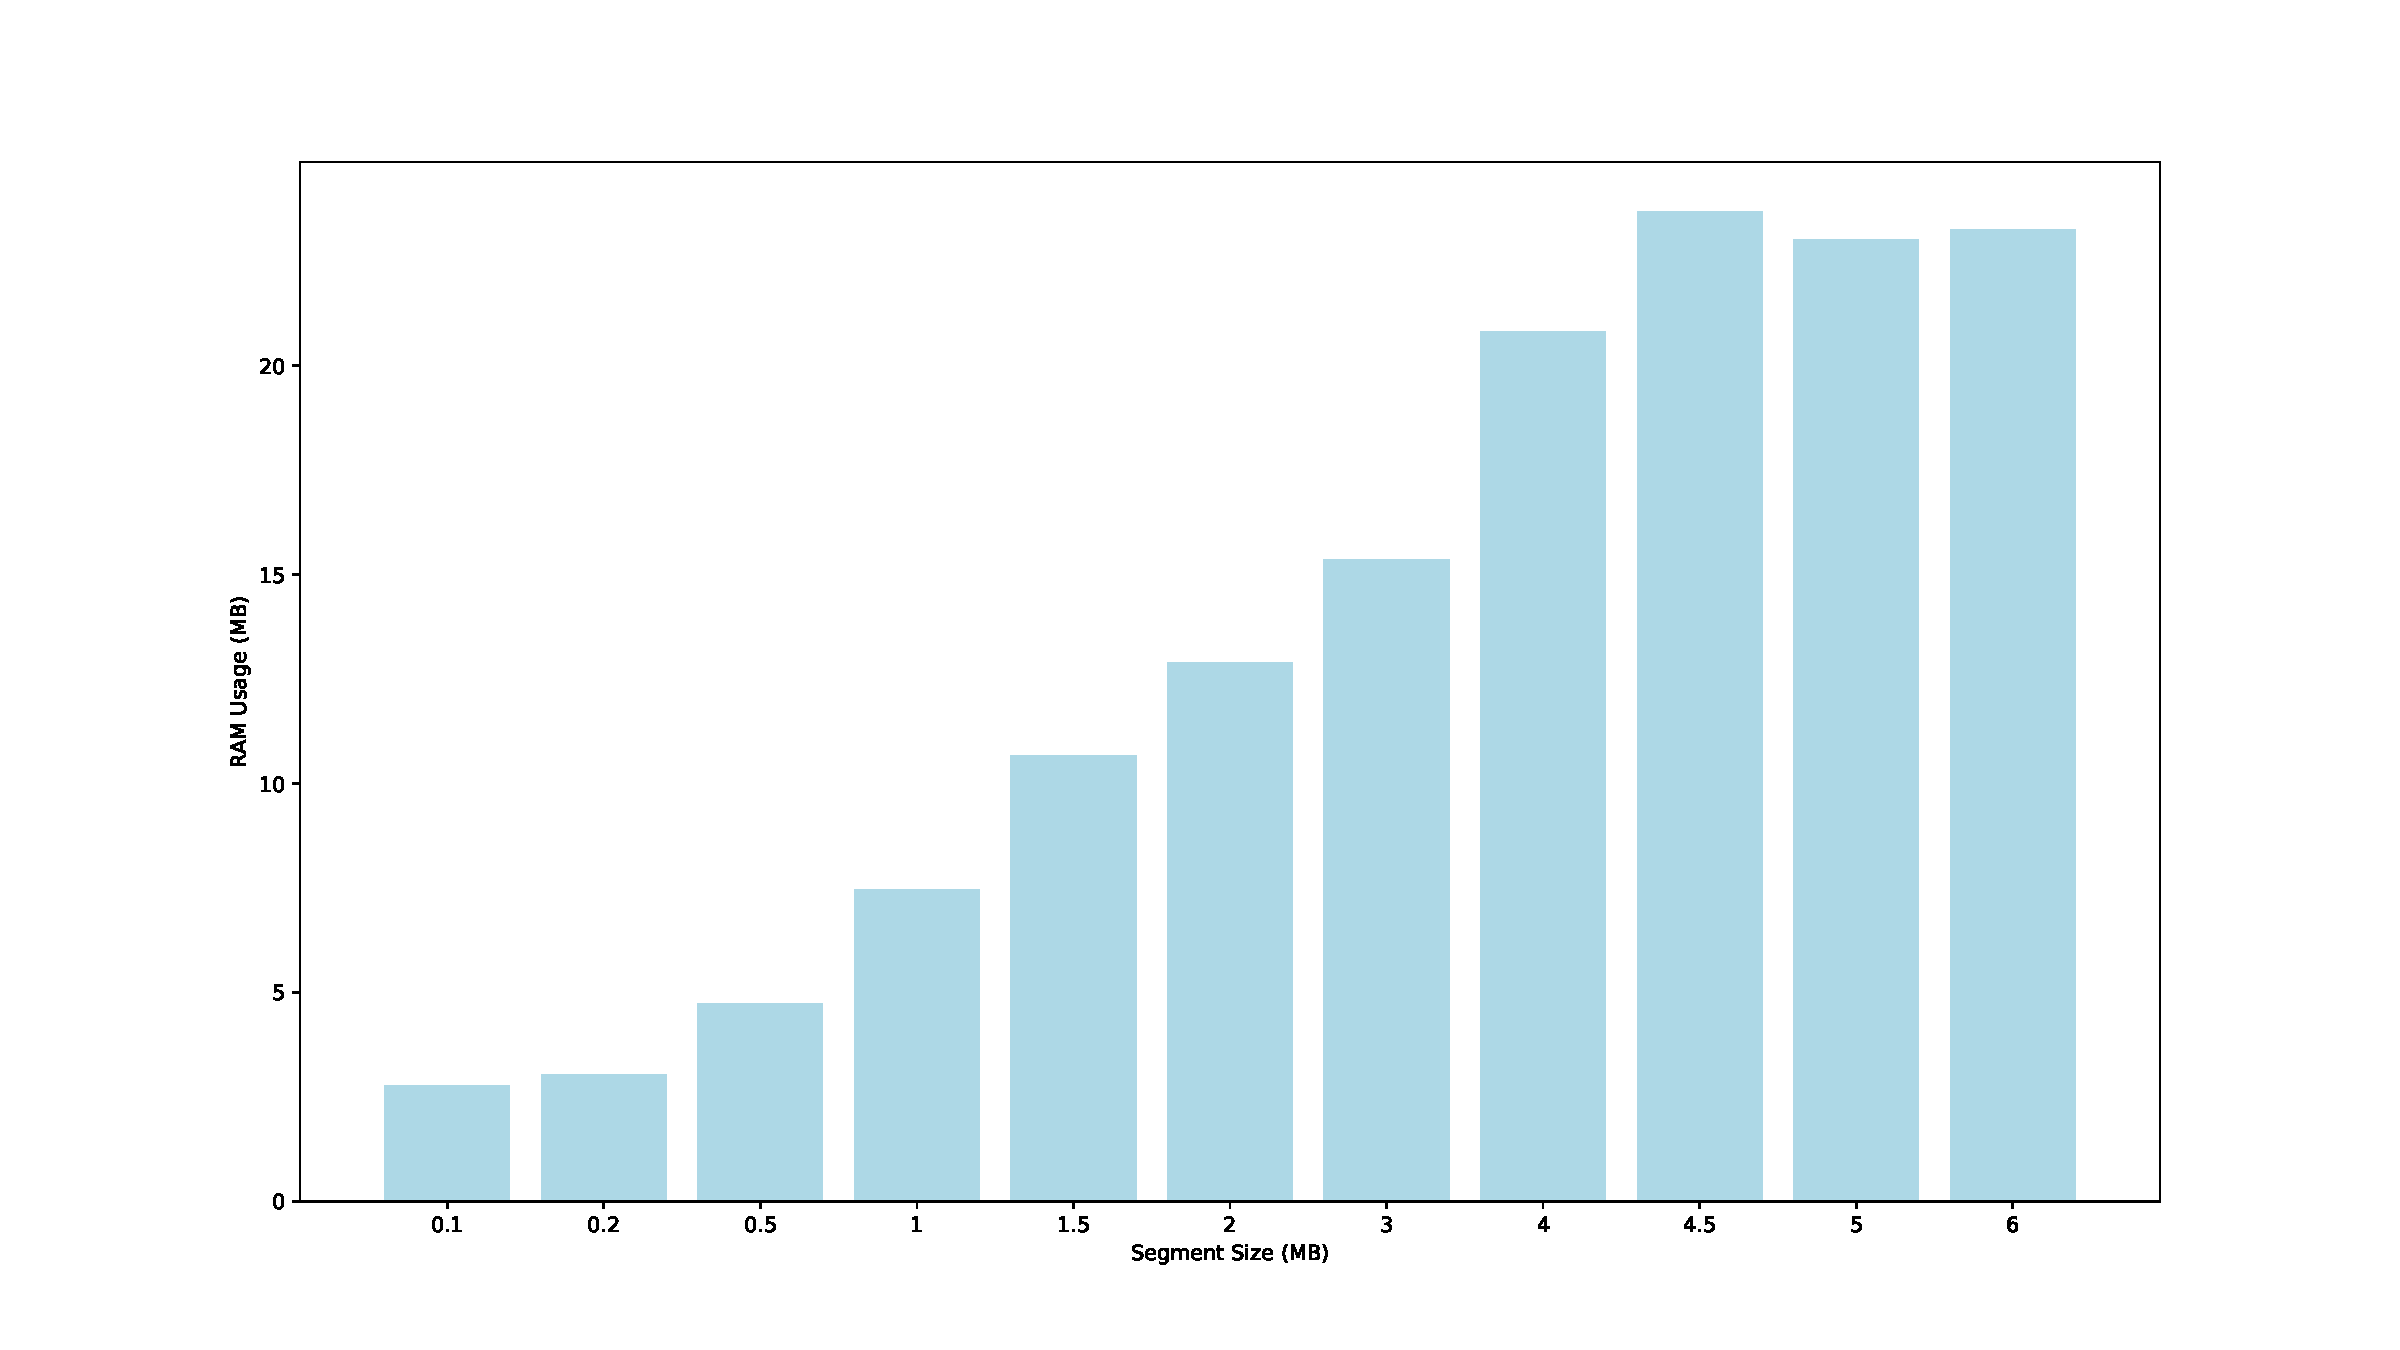
\includegraphics[width=1\linewidth]{content/figures/barplot_segsize.pdf}
\caption{RAM Memory usage for the healthcare synthetic log with 1000 traces}
\label{fig:barplot_segsize}
\end{figure}

\begin{figure}[t]
\centering
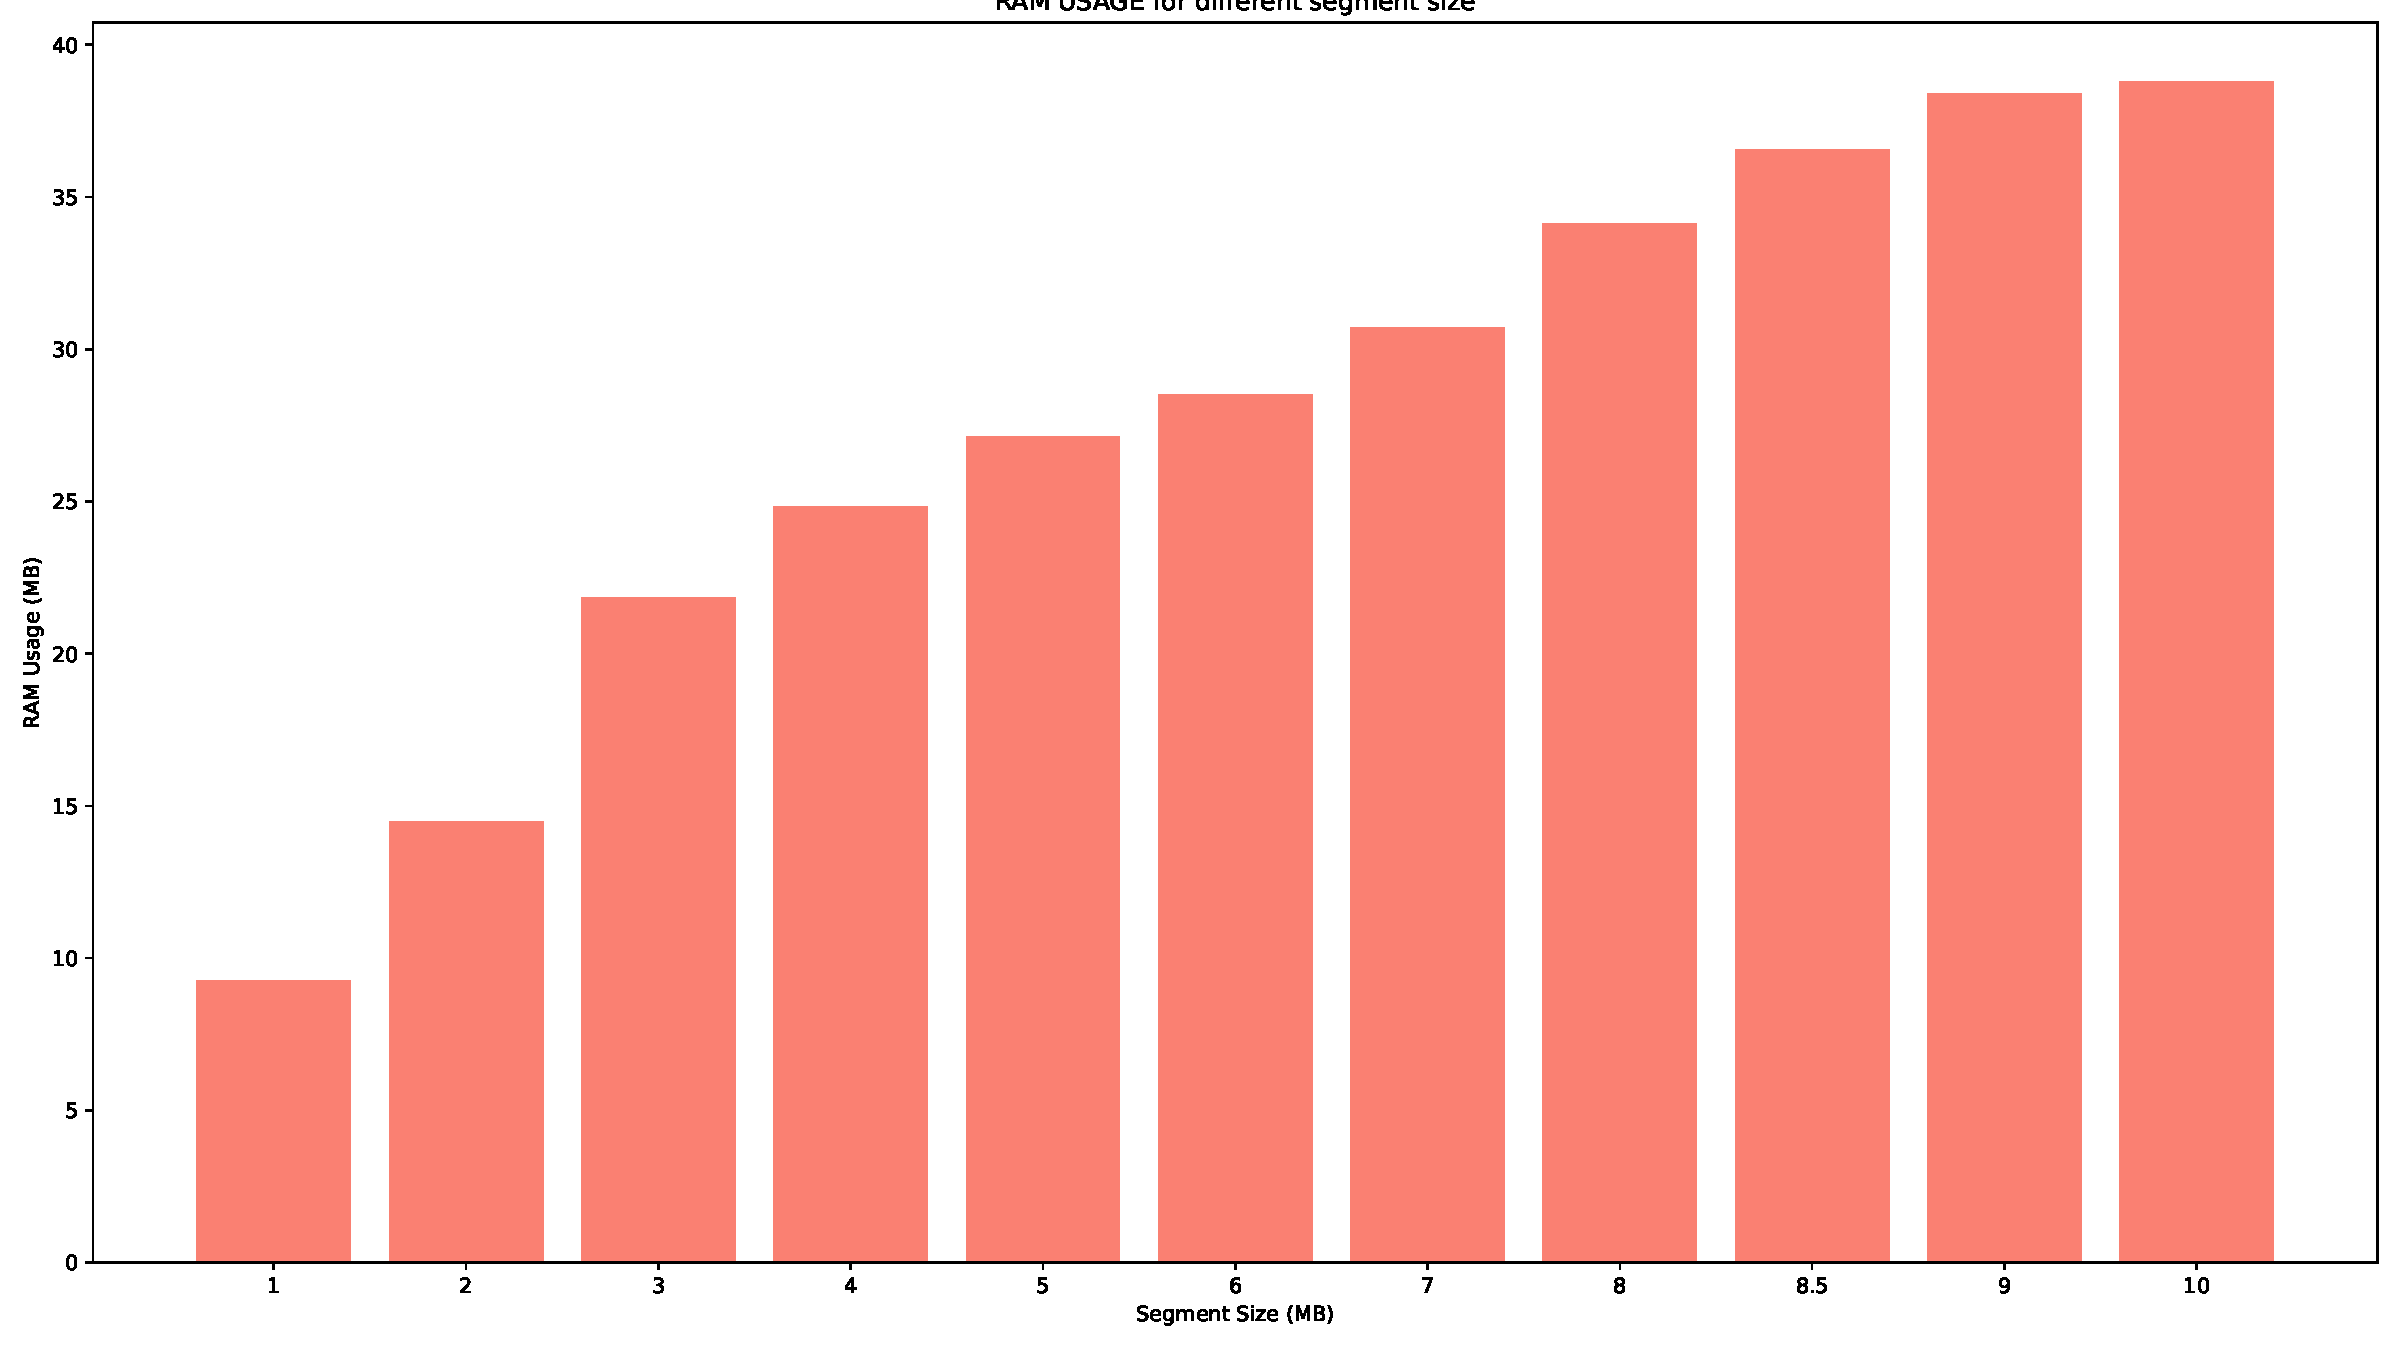
\includegraphics[width=1\linewidth]{content/figures/barplot_segsize_syth_2k.pdf}
\caption{RAM Memory usage for the healthcare synthetic log with 2000 traces}
\label{fig:barplot_segsize_synth_2k}
\end{figure}

\begin{figure}[t]
\centering
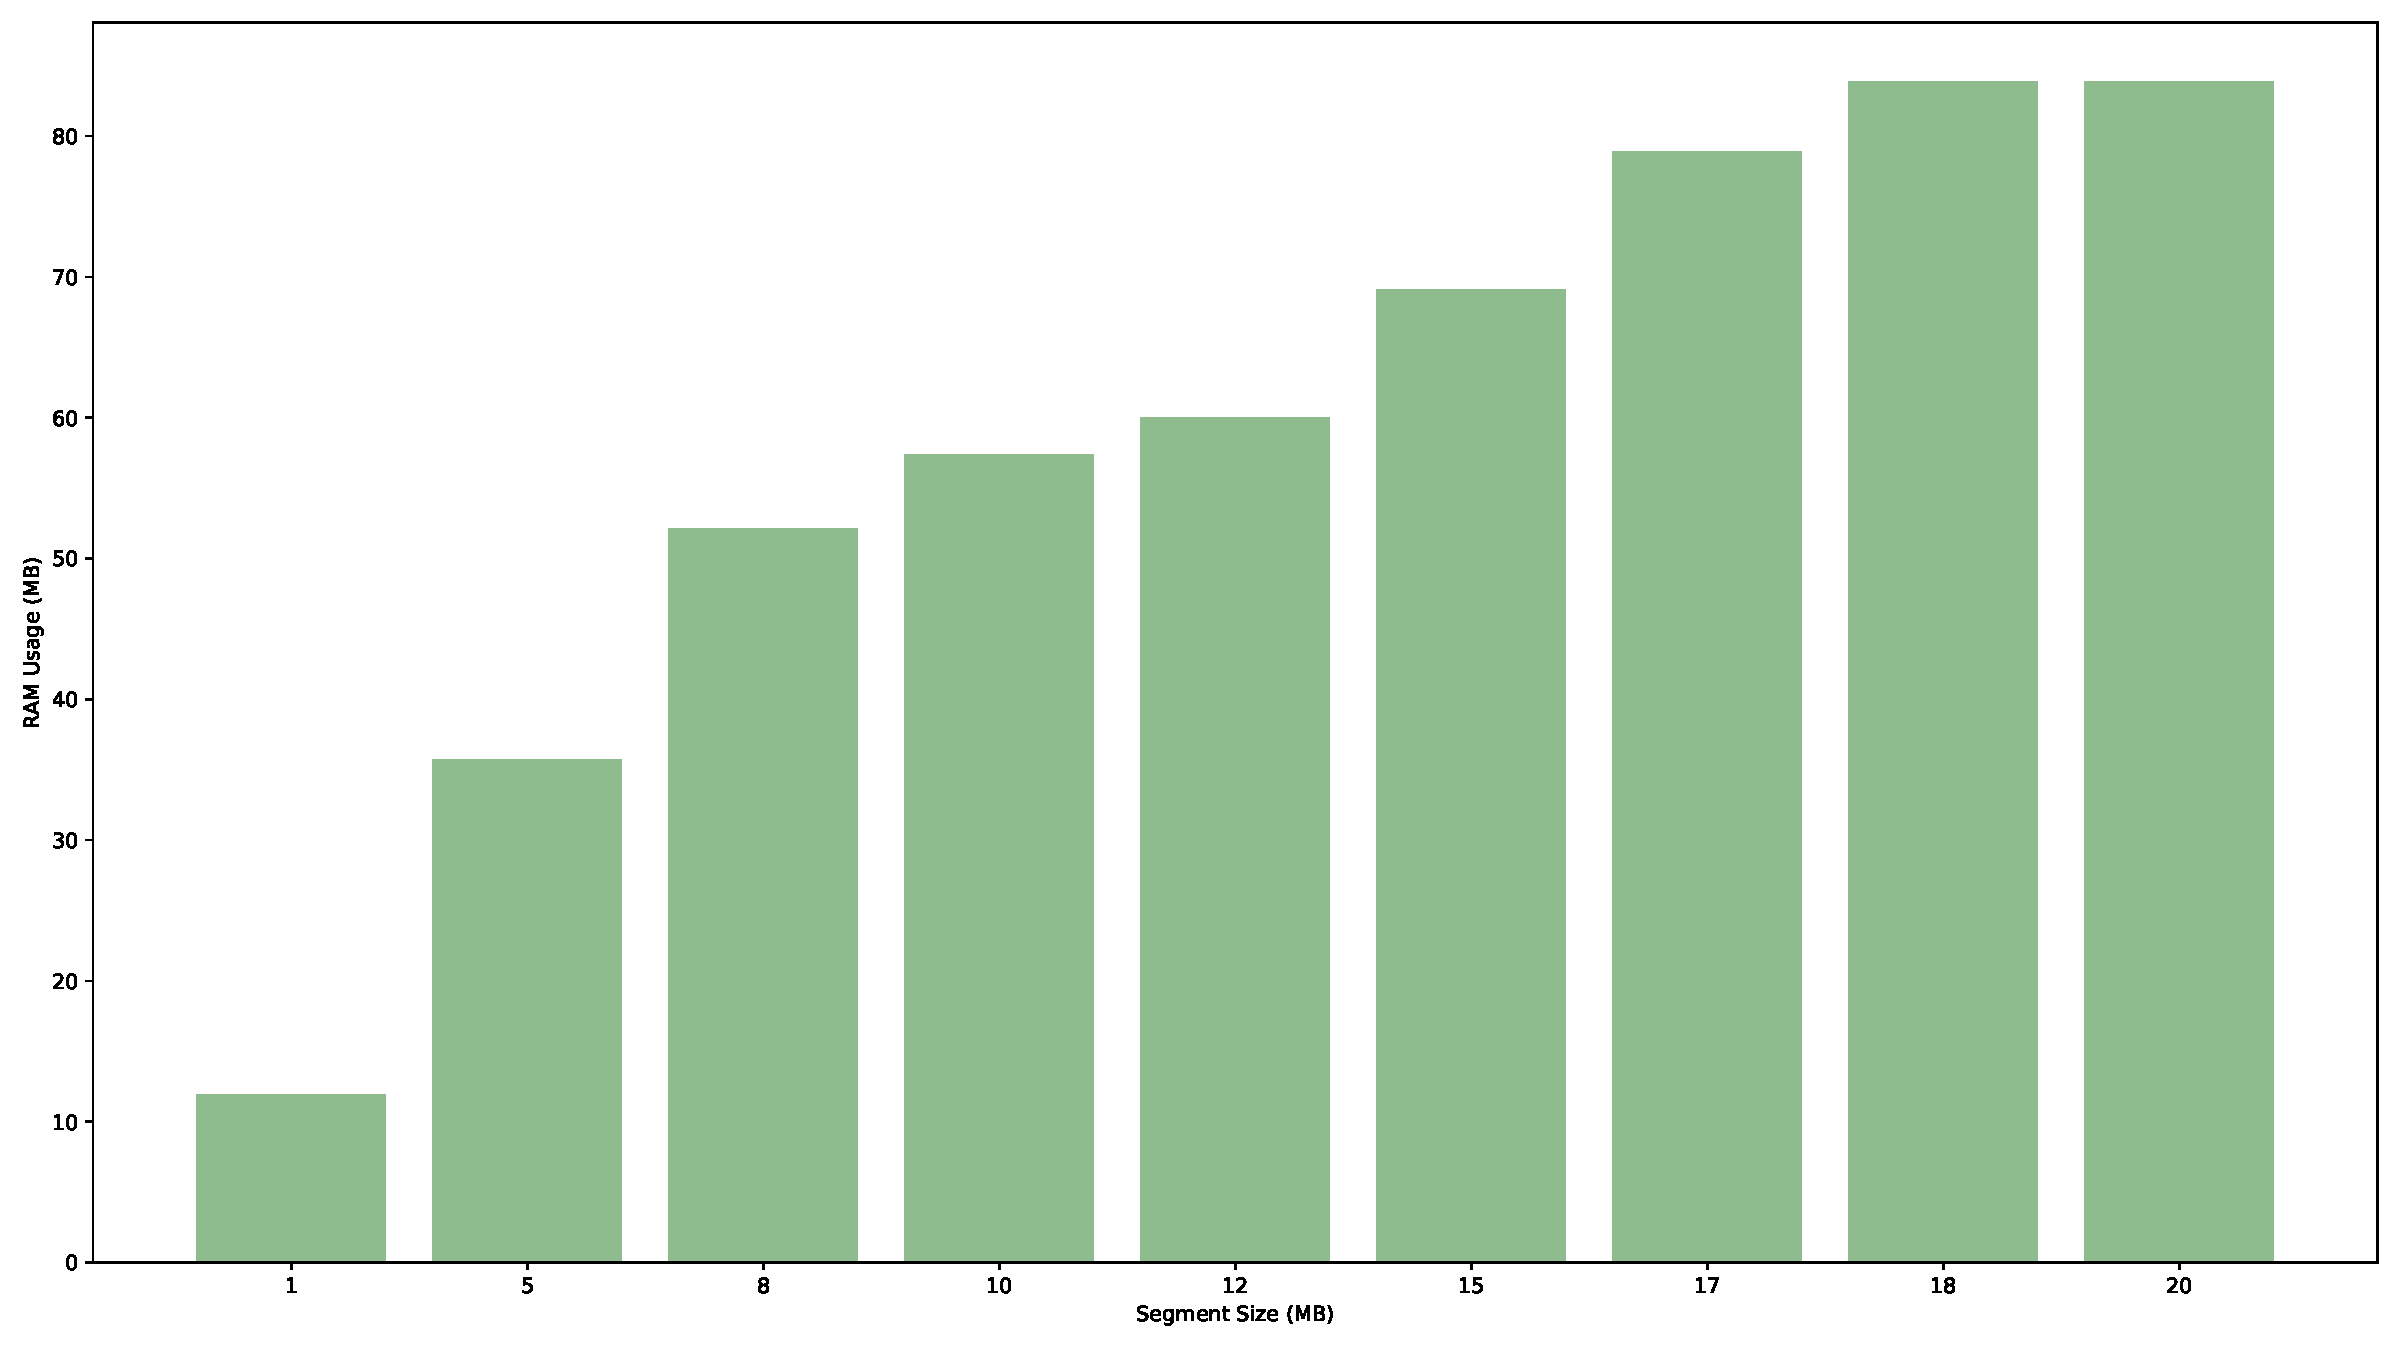
\includegraphics[width=1\linewidth]{content/figures/barplot_segsize_syth_4k.pdf}
\caption{RAM Memory usage for the healthcare synthetic log with 4000 traces}
\label{fig:barplot_segsize_synth_4k}
\end{figure}

\begin{figure}[t]
\centering
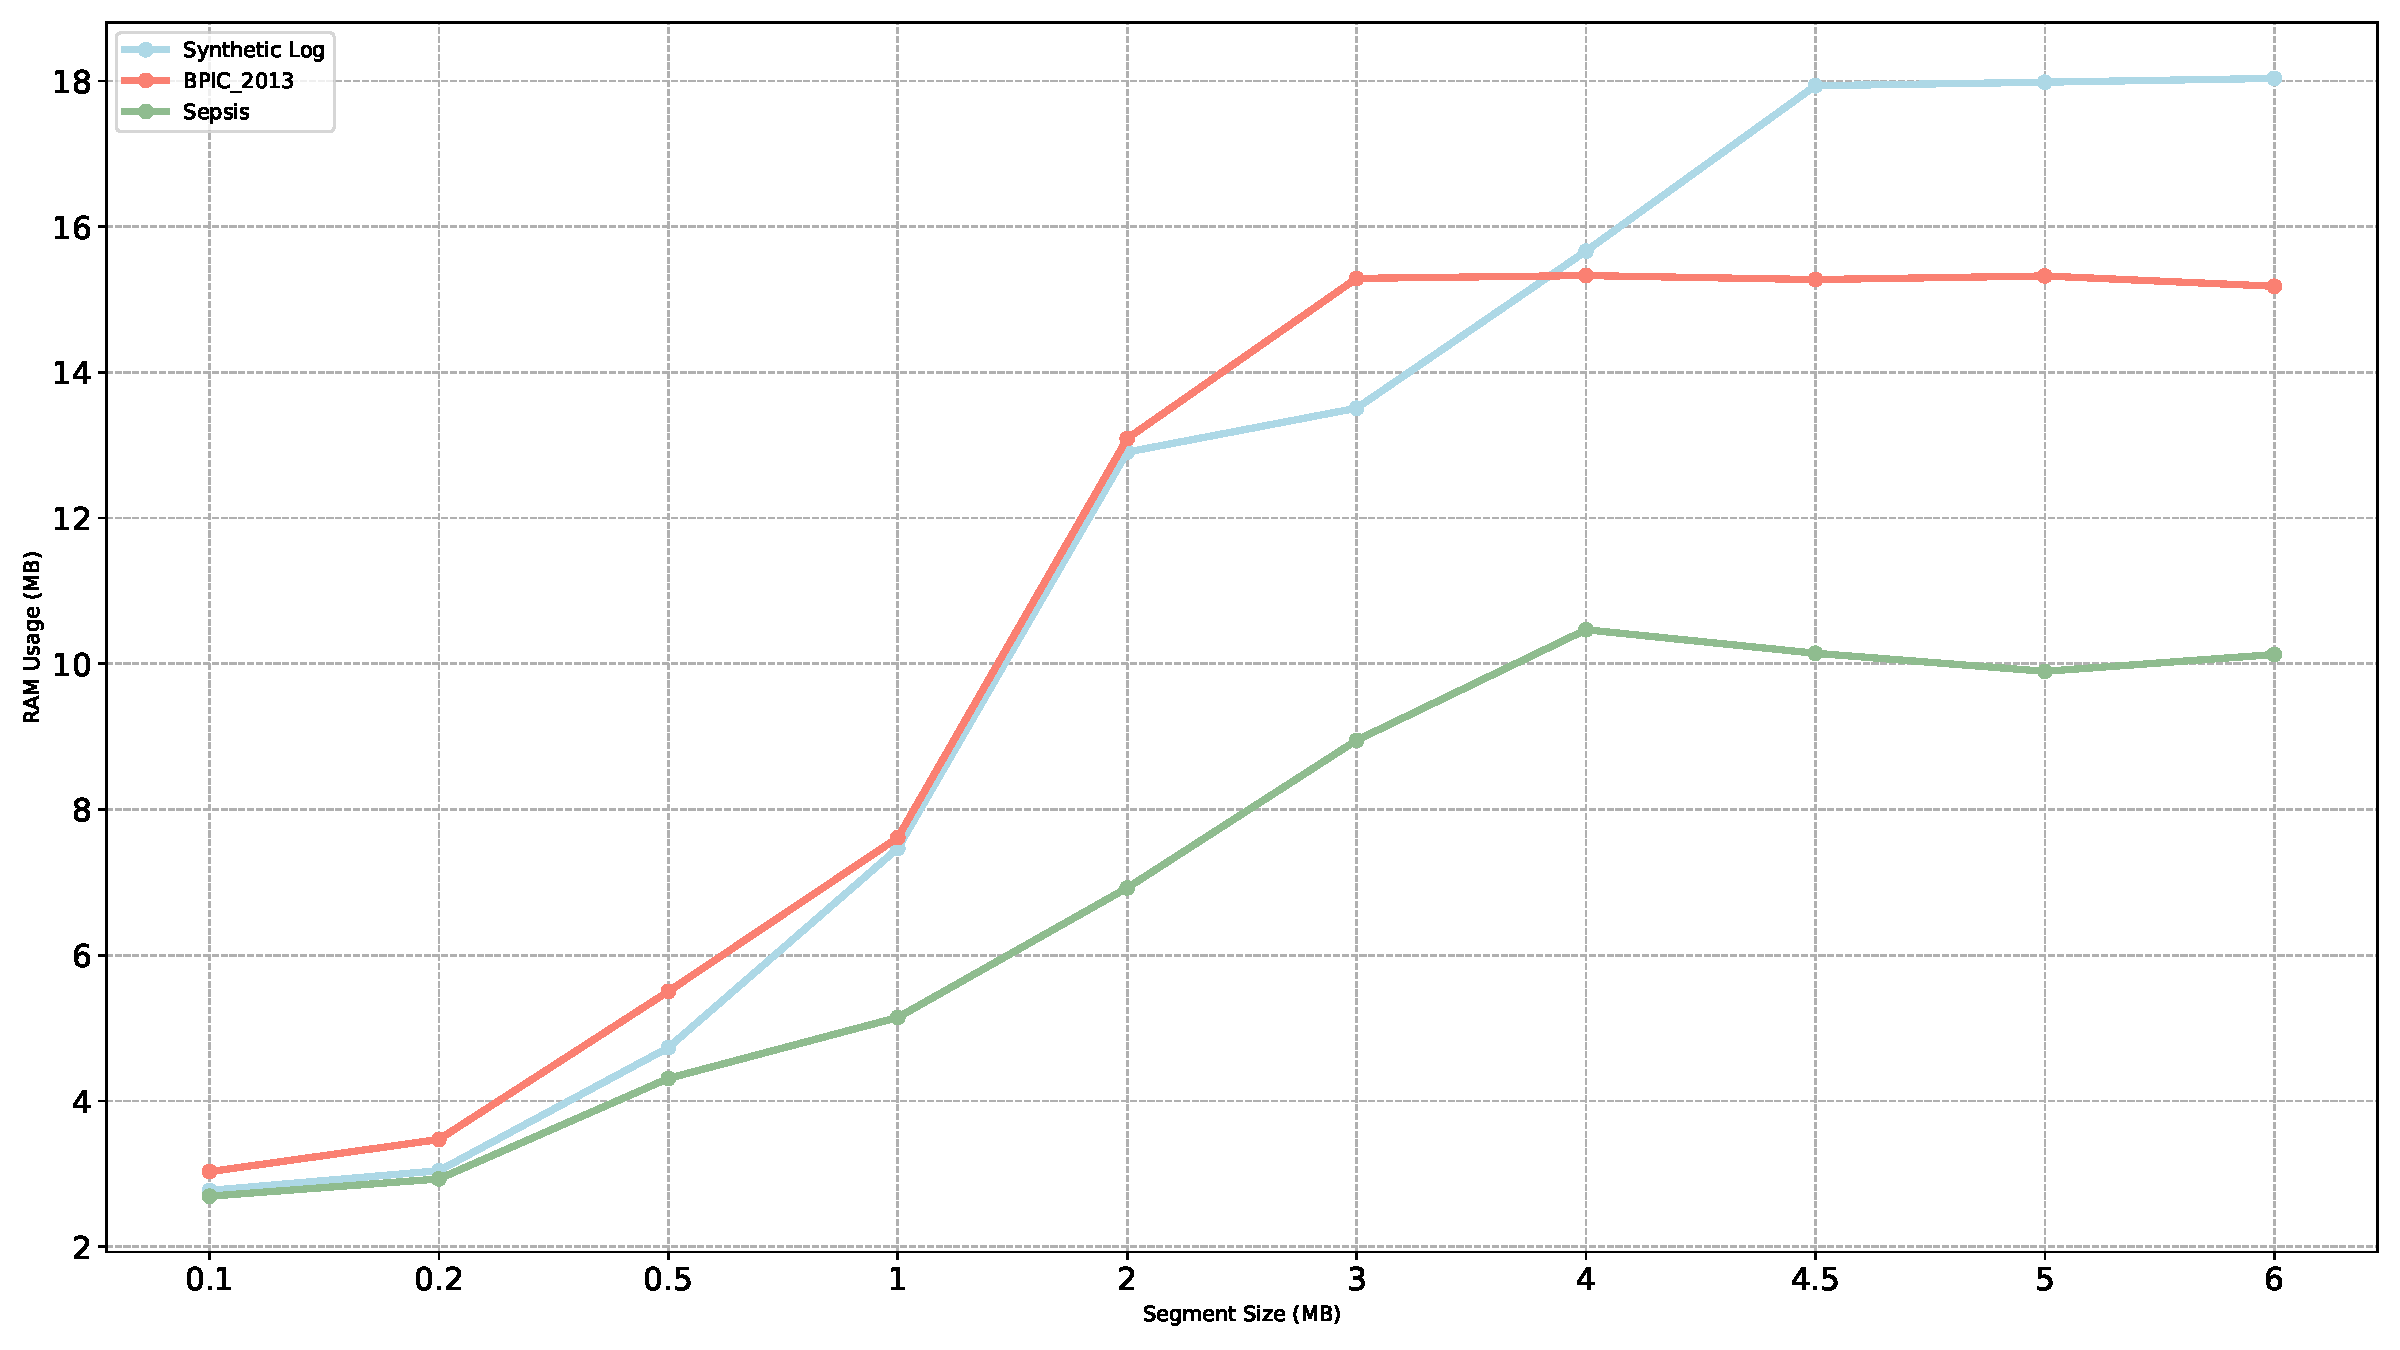
\includegraphics[width=1\linewidth]{content/figures/lineplot_segsize_combined.pdf}
\caption{RAM Memory usage for the synthetic log, BPIC 2013 and Sepsis Log}
\label{fig:lineplot_segsize_combined}
\end{figure}


\begin{figure}[t]
\centering
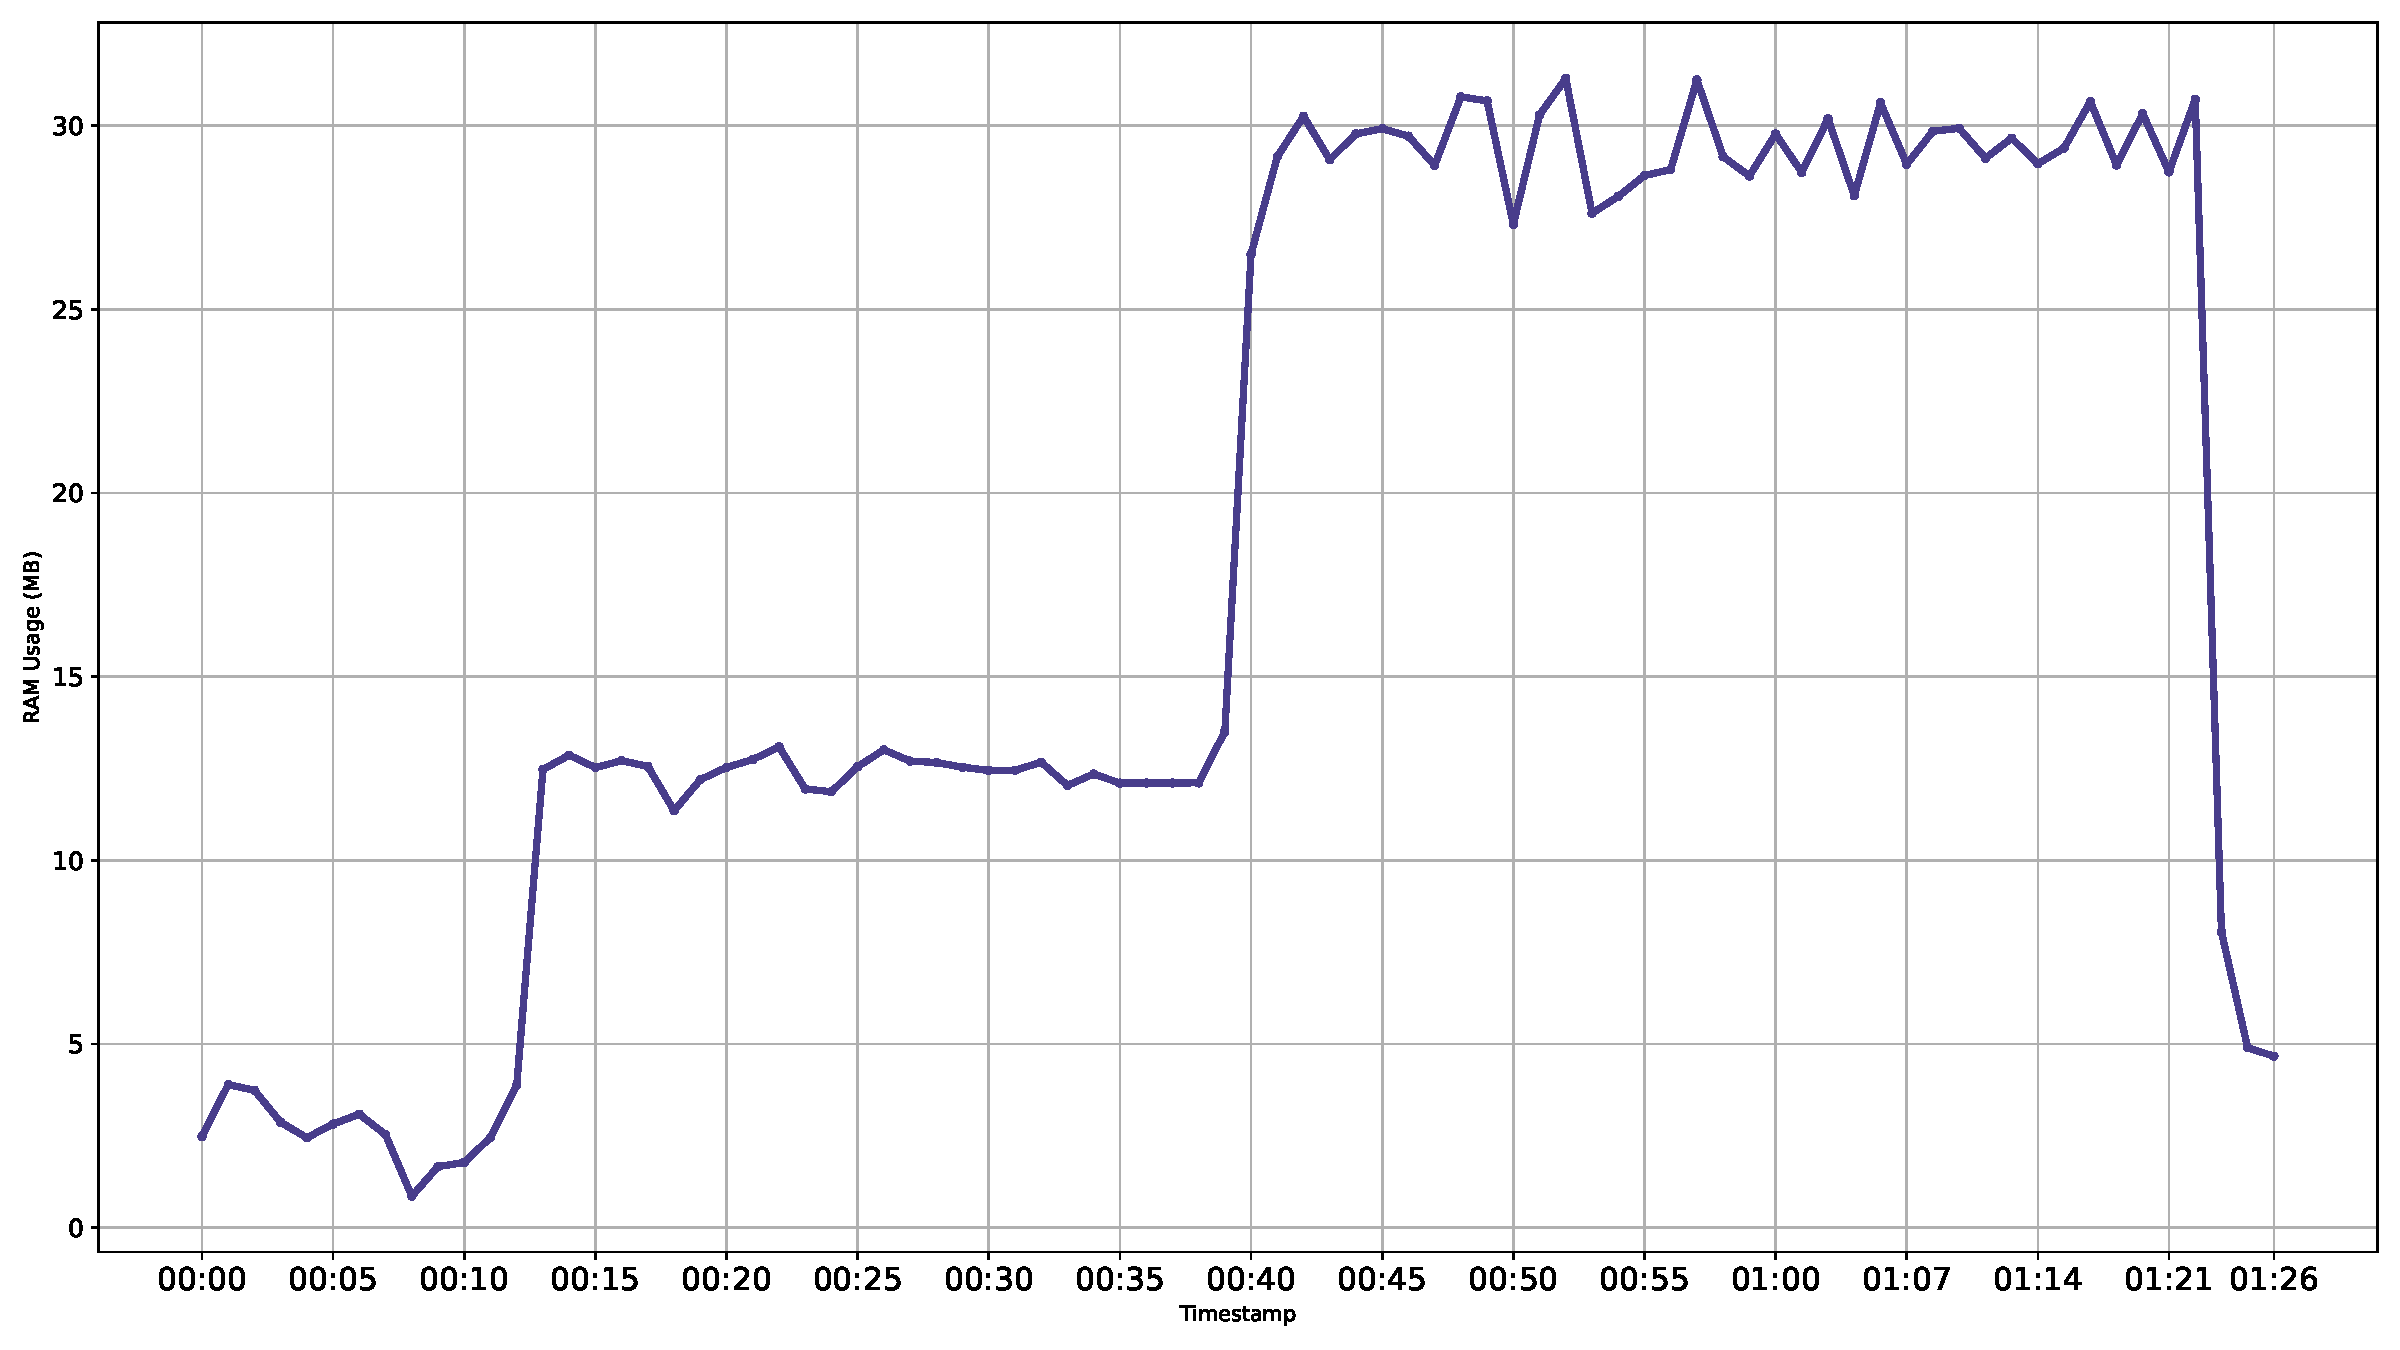
\includegraphics[width=1\linewidth]{content/figures/ram_usage_per_TS.pdf}
\caption{RAM Memory usage for a single run for the healthcare synthetic log with 1000 traces}
\label{fig:ramusage_ts}
\end{figure}


\subsection{Integrity and Confidentiality}
\label{sec:discussion:subsec:integrityandconfidentiality}
An essential aspect of the evaluation pertains to the fundamental principles of integrity and confidentiality upheld by the Trusted Execution Environment (TEE), crucial pillars that underpin the effectiveness and trustworthiness of the event log sharing mechanism. In this framework, the TEE is the cornerstone of data processing, demonstrating praiseworthy abilities to ensure data integrity. Throughout the entire process, from the moment data is ingested from individual organizations to the merging of event logs, the TEE maintains an unyielding grip on data integrity, steadfastly safeguarding against unauthorized modifications. This veracity is established through cryptographic hashing and secure storage mechanisms that ensure that the merged event log remains unaltered and representative of the original data. Concurrent with data integrity, the TEE exercises a robust commitment to confidentiality. The cryptographic measures implemented within the TEE ensure that all data, whether in transit or at rest, is encrypted with a level of security that mitigates the risk of unauthorized access. This cryptographic fortification guarantees that sensitive information encapsulated within event logs remains comprehensively shielded, rendering them inaccessible to any unauthorized entities. As a result, participating organizations can confidently share their event logs, knowing that their proprietary and sensitive information remains impervious to prying eyes.


\end{comment}
\section{Conclusion and Future Work}
\label{sec:conclusion}
Confidentiality is of paramount importance in inter-organizational process mining due to the transmission of sensitive data across organizational boundaries. Our research investigates a secrecy-preserving approach that enables organizations to employ process mining techniques with event logs from multiple organizations while ensuring the protection of privacy and confidentiality. Our solution still has room for improvement. We operate under the assumption of fair conduct by data provisioners and do not account for the presence of injected or maliciously manipulated event logs. In addition, we do not handle TEE crashes and suppose that miners and providers exchange messages in perfect communication channels where no loss, no snap, and no bit corruption occours. Additionally, our approach relies on certain assumptions about event log data, including the existence of a universal clock for event timestamps, which may not be realistic in situations where organizations are not perfectly synchronized. To address this challenge, we intend to explore a solution based on Network Time Protocols (NTP). Our future work encompasses the development of a formalized interaction protocol governing the communication between data provisioners and miners. The presented solution embraces model process mining techniques in a general way. However, we believe that the presented approach is particularly compatible with declarative model representations. Therefore, trusted applications could compute and store the entire set of rules representing a business process, and users may interact with them via trusted queries. Finally, in our implementation, we have focused on process discovery tasks. However, our approach has the potential to seamlessly cover a wider array of process mining functionalities such as \textit{conformance checking}, and \textit{performance analysis} techniques. Implementing them and show their integrability with our approach paves the path for future work. 
%\todo{CDC: The bibliography entries are too rich. Look at \cite{engel2011process}. Do we really care that the conference was in Toulouse? And look at \cite{koch2002expressive}: the acronym is enough for the conference name. Also, the volume number is useless if we do not have the series (anyway, we could not care less about either of the two). We have already gone through this, so we should shorten the entries as we know.}

\begin{comment}
Limitations:
\begin{itemize}
    \item Both producer and consumer act fairly (so we do not expect to have injected data) ok
    \item We do not manage TEE crashes
    \item We assume a perfect communication channel (no loss, no snap, no corrupted bits)
    \item Universal clock for event timestamps (cite Event log cleaning for business process analytics by Andreas Solti)
\end{itemize} 
Future Work:
\begin{itemize}
    \item Declarative models adaptation ok
    \item Output inside the TEE, interactions through trusted applications
    \item Real-world event log data ok
    \item Usage policies integration ok
    \item Formal interaction protocol ok
    \item Threat model ok
    \item Security evaluation ok
\end{itemize}
\end{comment}
%future work, quali segment portano al risultato attuale e farlo per ogni risultato intermedio -call valerio claudio 9-06-23

\noindent\textbf{Acknowledgments.} The authors thank Giuseppe Ateniese for the fruitful discussion and insights.
This research work was partly funded by MUR under PRIN grant B87G22000450001 (PINPOINT), by the Latium Region under PO~FSE+ grant B83C22004050009 (PPMPP), and by the EU-NGEU under the NRRP MUR grant PE00000014 (SERICS).
\todo[inline]{\textbf{EXTENSION PLAN}:\\
Extended introduction\\
Add Background Section\\
Add more related work\\
Modify the motivating scenario (and the design alongside the implementation) with more attributes.\\
Add Notation and formalization of event logs, merging, partitioning and segmentation\\
Add Soundness and completeness theorems\\
\textbf{Add threat model $\bigvee$}\\
\textbf{Full pseudocode of the protocol $\bigvee$}\\
More real-world event logs (plus two, at least) with associated tests\\
Add communication overhead v.\ segment size charts: elab time vs segment size; total time (incl.\ network) vs segment size.\\
%Add latency comparison between with TEE and without TEE settings (if we have a TEE)\\
Integrate declarative conformance checking (let it be with Janus or MINERful).\\
Modify conclusion\\
}


\vspace{-2ex}
%%%%%%%%%%%%%%%%%%%%%%%%%%%%%%%%%%%%%%%%%%%%%
% Biblography
%%%%%%%%%%%%%%%%%%%%%%%%%%%%%%%%%%%%%%%%%%%%%
\bibliographystyle{splncs04}
\bibliography{bibliography}


\end{document}
